%% =====================================================================
%% main-llmxive.tex — content-extracted llmXive wrapper
%% =====================================================================
%% Generated by scripts/extract_paper_content.py. The original paper
%% body is preserved; the venue-specific preamble (class, bundled .cls
%% files, custom packages) is DISCARDED and replaced with the llmxive
%% house style + a shim block that no-ops any venue-specific macros the
%% body still references.
%% =====================================================================
\documentclass{llmxive}


%% ── Packages forwarded from original preamble ─────────────────
\usepackage{url}
\usepackage{amsfonts}
\usepackage{amsmath}
\usepackage{amssymb}
\usepackage{amsthm}
\usepackage{algorithm}
\usepackage{algpseudocode}
\usepackage{graphicx}
\usepackage{tabularx}
\usepackage{listings}
\usepackage{wrapfig}
\usepackage{pifont}
\usepackage{multirow}
\usepackage[most]{tcolorbox}
\usepackage{natbib}

%% ── Shim layer (venue macros made into no-ops) ────────────────
\makeatletter
\providecommand{\TODO}[1]{}
\providecommand{\abscontent}{}
\providecommand{\absfont}{}
\providecommand{\acknowledgments}{\section*{Acknowledgments}}
\providecommand{\address}[1]{}
\providecommand{\affiliation}[1]{}
\providecommand{\aistatsfinalcopy}{}
\providecommand{\animategraphics}[5][]{\includegraphics[#1]{#3#4}}
\providecommand{\argmax}{\mathop{\mathrm{arg\,max}}}
\providecommand{\argmin}{\mathop{\mathrm{arg\,min}}}
\providecommand{\authornote}[1]{}
\providecommand{\authornotemark}[1][]{}
\providecommand{\authorrunning}[1]{}
\providecommand{\blfootnote}[1]{\footnote{#1}}
\providecommand{\bm}[1]{\boldsymbol{#1}}
\providecommand{\corresponding}{}
\providecommand{\correspondingauthor}[1]{}
\providecommand{\eg}{e.g.,\xspace}
\providecommand{\email}[1]{\href{mailto:#1}{#1}}
\providecommand{\equalcontribution}{}
\providecommand{\etal}{et al.\xspace}
\providecommand{\etc}{etc.\xspace}
\providecommand{\iclrfinalcopy}{}
\providecommand{\icmlfinalcopy}{}
\providecommand{\ie}{i.e.,\xspace}
\providecommand{\iid}{i.i.d.\xspace}
\providecommand{\institute}[1]{}
\providecommand{\keywords}[1]{\par\noindent\textbf{Keywords:} #1}
\providecommand{\neuripsfinalcopy}{}
\providecommand{\orcid}[1]{}
\providecommand{\tablecite}[1]{\cite{#1}}
\providecommand{\theabstract}{}
\providecommand{\titlerunning}[1]{}
\providecommand{\todo}[1]{}
\providecommand{\wrt}{w.r.t.\xspace}
\AtBeginDocument{\renewcommand{\and}{ \textperiodcentered\ }}
\makeatother

%% ── User-defined macros forwarded from original preamble ─────
\makeatletter
\providecommand{\ours}{\texttt{BES}}
\providecommand{\arraystretch}{1.20}
\definecolor{cellbase}{HTML}{F9F9F9}
\definecolor{tabband}{HTML}{F2F7FB}
\definecolor{darkerlogocolor}{RGB}{20, 0, 145}
\newtcolorbox{ttcolorbox}[1][]{
  colframe=darkerlogocolor,
  colback=darkerlogocolor!4!white,
  title=#1,
  breakable,
  enhanced jigsaw,
}
\makeatother

%% ── llmXive paper metadata ──────────────────────────────────
\title{Self-Improving Language Models with Bidirectional Evolutionary Search}
\author{Guowei Xu \and Zhenting Qi \and Huangyuan Su \and Weirui Ye \and Himabindu Lakkaraju \and Sham M. Kakade \and Yilun Du}
\paperid{arXiv:2605.28814}
\paperstatus{Preprint}

\begin{document}
\maketitle
\begin{abstract}
Search has been proposed as an effective method for self-improving language models and agentic systems, both for post-training sample generation and for inference. However, widely used methods such as best-of-N sampling and tree search face two fundamental limitations: they are guided by sparse verification signals, and they construct candidates primarily through autoregressive expansion, restricting exploration to regions with substantial model probability mass. To address these, we propose Bidirectional Evolutionary Search (\ours), a search framework that couples forward candidate evolution with backward goal decomposition. In the forward search, \ours\ augments standard expansion with evolution operators that recombine partial trajectories to generate candidates that are difficult to obtain from a single model rollout. In the backward search, \ours\ recursively decomposes the original task into checkable sub-goals, producing dense intermediate feedback that guides forward search. We provide theoretical motivation showing that candidates generated by expansion-only search are confined to a narrow entropy shell while evolutionary operators can escape it, and that backward search can exponentially reduce the number of required samples to find a correct answer. Experiments show that on challenging post-training tasks where mainstream post-training algorithms fail to improve, \ours\ enables consistent gains, and on three open problem solving benchmarks at inference time, \ours\ outperforms existing open-source frameworks in both average and best-case performance. Code and trained models are available at \url{https://github.com/Embodied-Minds-Lab/BES}.
\end{abstract}
\etocdepthtag.toc{mainpaper}


\section{Introduction}
Large language models (LLMs) and agentic systems have demonstrated remarkable capabilities on complex reasoning problems~\citep{cot, rstar, dsr1}. They can even solve open problems across mathematical and scientific domains~\citep{alphaevolve,alphaproof} and surpass the best human performance on tasks such as code generation~\citep{alphacode, tttdiscover}. In this context, the question of how to do better sampling from LLMs and agentic systems is of critical importance~\citep{rstarmath}. This is particularly significant for problems at the frontier of model capability, where naive sampling methods may require too many samples to obtain a correct answer or may simply fail~\citep{frontiermath,rlincentivize}. At training time, higher-quality samples enable more effective post-training and self-improvement~\citep{star,selfreward}; at inference time, they serve as a natural mechanism for test-time scaling~\citep{selftaught, wu2025inference, shinkaevolve}, which can further push the boundary of what models can achieve.

Currently, the two dominant sampling methods in post-training, self-improvement, and inference for LLMs and agentic systems are best-of-N sampling and tree search. Best-of-N sampling is simple and efficient. For problems of moderate difficulty, it typically suffices to find high-quality responses and is therefore widely adopted in post-training algorithms such as GRPO~\citep{dsr1} and its variants~\citep{dapo}, while also serving as a strong baseline for inference. Tree search methods such as beam search and Monte Carlo Tree Search~\citep{mcts} can discover better responses more sample-efficiently than best-of-N on harder problems. For example, Tree-GRPO leverages tree search for sample generation during post-training~\citep{treegrpo}, and Tree of Thoughts explores multiple reasoning paths at inference time~\citep{tot}.

However, both methods share two fundamental limitations.  (1) The verification signal to guide the search is sparse. Effective search depends critically on the accuracy and granularity of the verifier, yet in common settings such as RLVR post-training, verifiers typically provide only binary or coarse-grained feedback. (2) They struggle to generate candidates beyond the model's own distribution. They construct candidates by auto-regressively extending responses. This confines candidates to the support of the model's own distribution~\citep{llmmonkey}, making it difficult to reach low-probability regions where correct solutions often reside on hard problems.

\begin{figure}[t]
\centering
\vspace{-1em}

\includegraphics[width=\linewidth]{images/teaser.pdf}
\vspace{-1em}
\caption{Comparison of tree search and Bidirectional Evolutionary Search (\ours). \textbf{Left:} Tree search constructs candidates by sequentially expanding steps. We prove that all such candidates are confined to a narrow entropy shell (Theorem~\ref{thm:shell}a), limiting exploration to a small region of the solution space. \textbf{Right:} \ours\ escapes this shell through evolution operators that recombine
parts of different trajectories, with backward search decomposing the
problem into verifiable sub-goals that provide dense feedback to guide
the forward search toward the final goal. \checkmark and {$\boldsymbol{\times}$} indicate whether a candidate satisfies or fails the (sub-)goal, respectively.}
\vspace{-2em}
\label{fig:teaser}
\end{figure}

To address these two limitations, we propose  Bidirectional Evolutionary Search (\ours). First, to tackle the sparsity of verification signals, we introduce bidirectional search: the forward search seeks better candidate solutions, while the backward search discovers finer-grained sub-goals to verify them.
Second, to generate candidates beyond the model's own distribution, we draw inspiration from evolutionary biology. 
For much of the history of life, organisms reproduced asexually. Each offspring was a direct extension of its parent, and beneficial mutations arising independently in different individuals could never be combined~\citep{naturalselection}. Sexual reproduction fundamentally changed this through chromosomal recombination: gene segments from different lineages are spliced together to produce novel combinations that neither parent possessed~\citep{sex}. Analogously, in our setting, rather than only extending responses auto-regressively, we introduce four evolution operators: combination, translocation, deletion, and crossover. Combination, translocation, and crossover merge the strengths of two distinct responses in different ways to construct a new candidate, while deletion removes the least sound segment from a response. We theoretically prove that responses generated by expansion-only search are confined to a narrow entropy shell, while evolution operators can escape it.

We evaluate \ours\ on both post-training and inference across LLM and agent settings. For post-training, we test on challenging logical reasoning and multi-hop reasoning tasks where mainstream post-training algorithms such as GRPO~\citep{dsr1}, MaxRL~\citep{maxrl}, and Tree-GRPO~\citep{treegrpo} struggle to find sufficient high-quality training samples and consequently fail to improve or even degrade from the base model. In contrast, \ours\ consistently discovers effective training samples, enabling meaningful improvements where these baselines nearly fail. For inference, we test on three open problem solving benchmarks, where \ours\ discovers more stable and higher-quality solutions compared to all existing open-source frameworks, including OpenEvolve~\citep{openevolve}, GEPA~\citep{gepa}, and ShinkaEvolve~\citep{shinkaevolve}. We also provide ablation studies validating the contribution of each component, case studies visualizing our search process, and cost analysis comparing the wall-clock time and API cost of \ours\ against baselines.

\section{Preliminaries}
\label{sec:problem}

We consider reasoning problems of the form
$
  \mathcal{T} = (x, V),
$
where $x$ is a problem description (e.g.\ a math question) and
$V(x,y) \in [0,1]$ is a \emph{verifier} that
assigns a score measuring how well a trajectory $y$
solves the problem $x$.

Given a policy $\pi_\theta(\cdot\mid x)$ (e.g.\ an LLM that generates reasoning traces, or an agent that interacts with an environment through a sequence of actions), our goal is to produce a terminal response $y$ that maximizes the verifier score. Let
$\mathcal{Y}_{\mathrm{term}}(x)$ denote the set of valid terminal responses
under the task specification and resource budget. We write the target as
\begin{equation}
  y^{\star}(x) \;\in\; \operatorname*{arg\,max}_{y\in\mathcal{Y}_{\mathrm{term}}(x)}
                       V(x, y).
  \label{eq:obj}
\end{equation}
Finding $y^{\star}$ is important in both training and inference. During
training, high-quality candidates can facilitate post-training or
iterative self-improvement. During inference, $y^{\star}$ is the response
we seek.

The challenge is that the maximization in Eq.~\eqref{eq:obj} is intractable:
on hard problems, the probability mass that $\pi_\theta$ assigns to correct
trajectories can be extremely small. Practical algorithms therefore
approximate $y^{\star}$ by searching over a set of candidates. We 
introduce two common methods below.

\textbf{Best-of-$N$ sampling.}
The simplest approach is to draw $N$ independent trajectories and return the one with the highest verifier score. Formally, let $y^{(1)}, \dots, y^{(N)} \overset{\text{i.i.d.}}{\sim} \pi_\theta(\cdot \mid x)$. The method returns $ y^{\mathrm{BoN}} \;=\; \operatorname*{arg\,max}_{y \in \{y^{(1)}, \dots, y^{(N)}\}} V(x, y) $.
Best-of-$N$ is parallel and requires no structural knowledge of the problem. Its effectiveness, however, is bounded by the finite-sample coverage of $\pi_\theta$: all $N$ trajectories are drawn from the same distribution, so if the optimal trajectory lies in a region with very small policy mass, increasing $N$ gives only linear coverage improvement.

\textbf{Tree search.}
Tree-search methods exploit the sequential structure of a trajectory. A trajectory
is decomposed into steps (e.g.\ tokens, reasoning segments, or agent actions), and the
search maintains a tree whose nodes are partial trajectories and whose edges
correspond to appending a step. Branches are selected and extended according
to a heuristic value so that compute is concentrated on prefixes that look
promising. Classic methods include beam search, best-first search, and Monte
Carlo Tree Search~\citep{mcts}; recent work applies these ideas to LLM and agent reasoning~\citep{tot,treegrpo}. Tree search can be more sample-efficient than best-of-$N$
when the per-step signal is informative, but it still materializes terminal
candidates one lineage at a time through sequential extension.



\section{\ours: Bidirectional Evolutionary Search}
\label{sec:method}

 \ours\ performs a bidirectional evolutionary search that alternates
between two coupled processes: a \emph{forward} search that seeks
better candidates, and a \emph{backward} search that decomposes
the problem into fine-grained sub-goals to evaluate each forward
node. The forward search not only extends trajectories but also
recombines parts of different candidates, producing solutions that
no single rollout from $\pi_\theta$ would likely reach. The backward
search provides dense and interpretable scores for partial
trajectories, guiding the forward search toward promising
candidates. In practice, one backward search step is performed after every
several forward search steps. The full pseudocode is given in
Appendix~\ref{app:algo}, and a case study illustrating the search
process is provided in Appendix~\ref{app:case}.

\subsection{Forward Search: Expanding the Reachable Solution Space}
\label{sec:forward}

\begin{figure}[t]
\centering
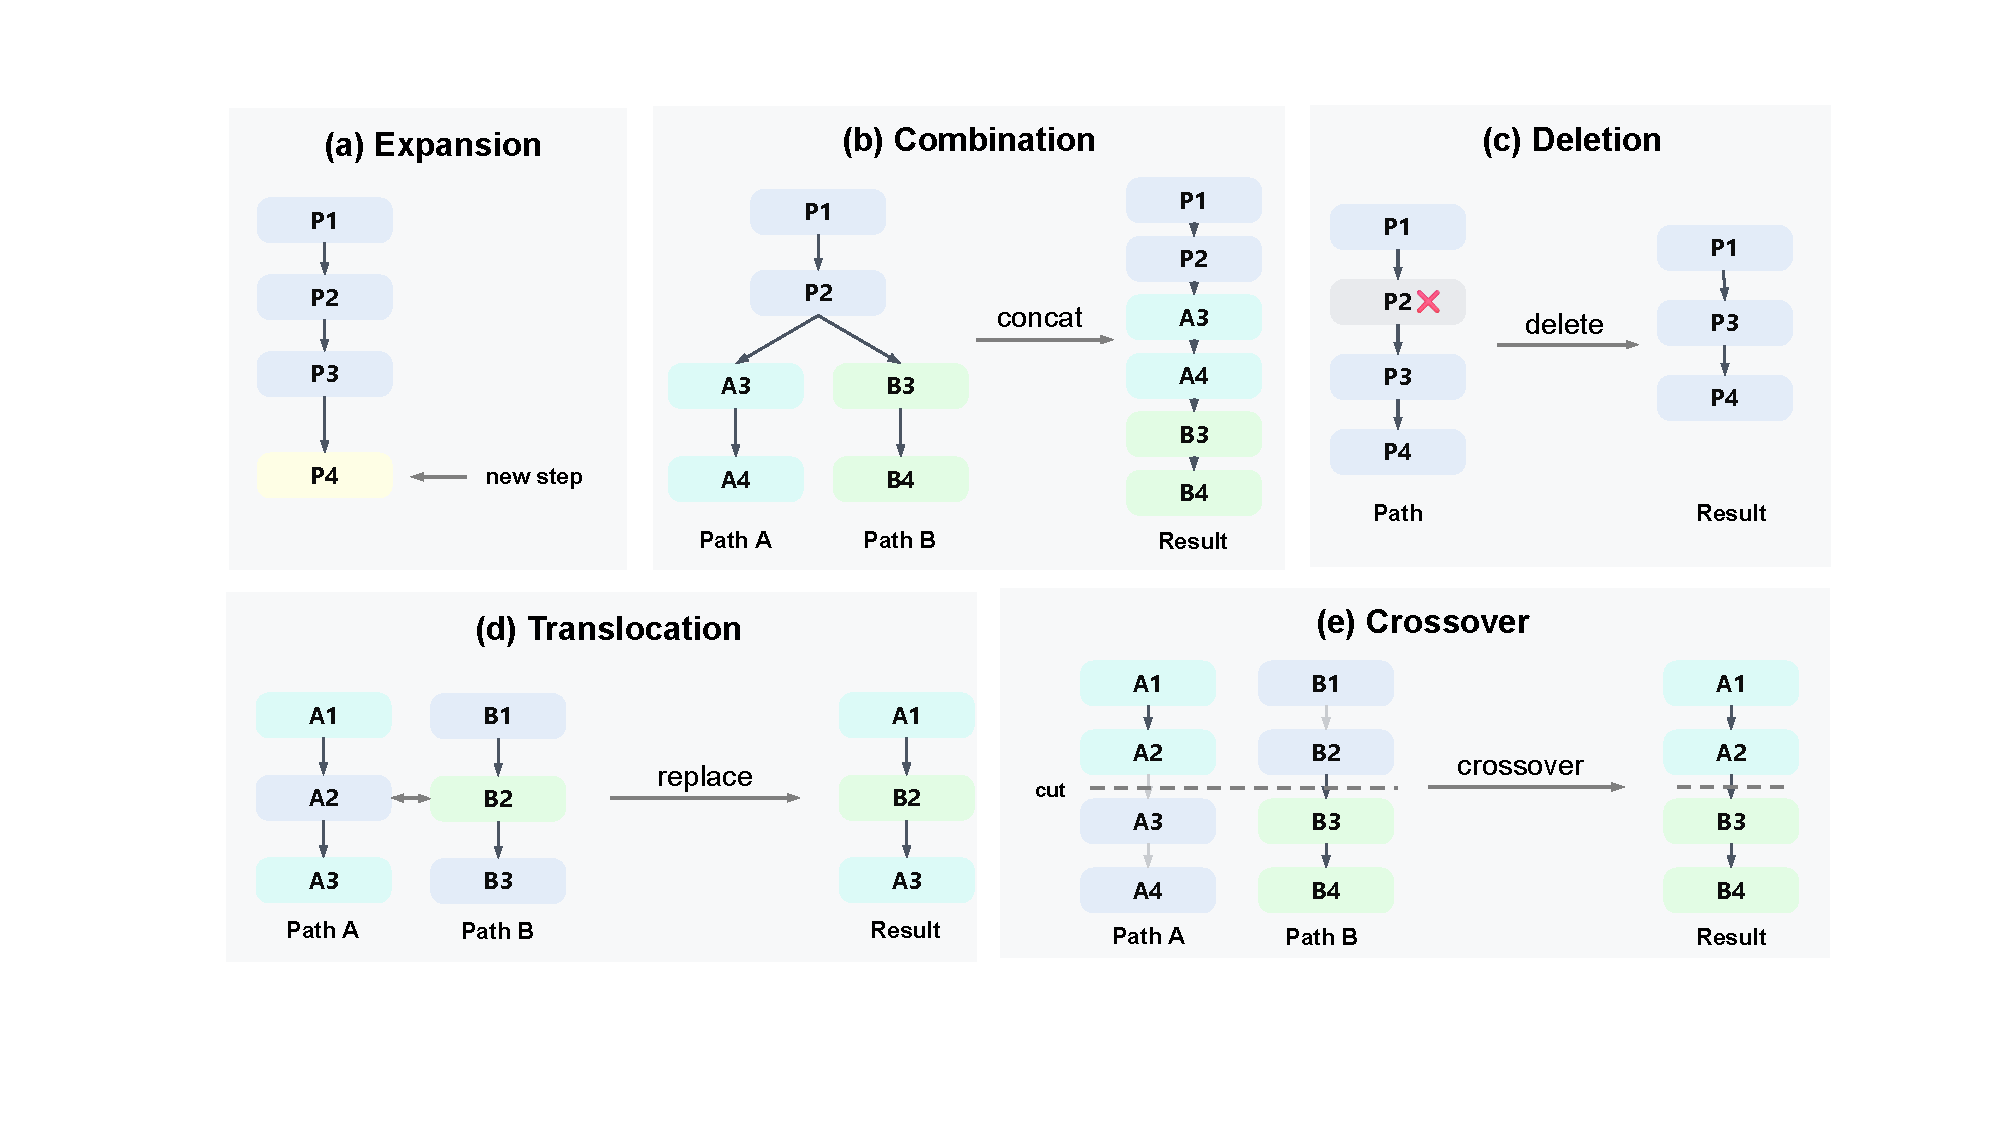
\includegraphics[width=\linewidth]{images/forward.pdf}
\caption{Forward search operators. \textbf{(a) Expansion:} the policy generates new steps (yellow). \textbf{(b) Combination:} two trajectories sharing a common prefix (P1--P2) have their distinct suffixes concatenated into a single candidate. \textbf{(c) Deletion:} an interior step (P2) is removed. \textbf{(d) Translocation:} one step in Path A (A2) is replaced by a step from Path B (B2). \textbf{(e) Crossover:} Path A is cut at a splice point and its tail is replaced by the tail of Path B. }
\vspace{-1em}
\label{fig:forward}
\end{figure}

We represent each candidate partial trajectory as a node
$n=(y_1,\dots,y_{t})$, where $y_i$ denotes the $i$-th step (e.g.\ a reasoning segment or an action). The search maintains a candidate set $\mathcal{P}$ of such nodes, and at
each search step applies one of two types of operators, \emph{expansion}
or \emph{evolution}, to produce a child node $n'$, which is scored by
the backward search (Section~\ref{sec:backward}) and added to $\mathcal{P}$.


\textbf{Expansion.}
Expansion extends a parent node by sampling new steps. Given
$n=(y_1,\dots,y_{t})$, we sample a step count
$K\sim\mathrm{Uniform}\{1,\dots,K_{\max}\}$ and draw up to $K$ new steps from
$\pi_\theta$:
\begin{equation}
  y_{t+k}\,\sim\,\pi_\theta\bigl(\cdot\mid x\oplus y_1\oplus\cdots\oplus y_{t+k-1}\bigr),
  \qquad k=1,\dots,K,
  \label{eq:expand}
\end{equation}

\textbf{Evolution.} 
 A key limitation of expansion alone is that each candidate
is built by sequentially extending a single trajectory,
so it cannot combine useful parts from different candidates.
Evolution operators overcome this by editing and recombining
existing trajectories. As illustrated in Figure~\ref{fig:forward}, we define four operators inspired by biological evolution: \textit{(i) Combination} merges two trajectories by concatenating their suffixes beyond a shared prefix; \textit{(ii) Deletion} removes one interior step, producing a shorter candidate; \textit{(iii) Translocation} transplants a single step from one trajectory into another; and \textit{(iv) Crossover} splices the prefix of one trajectory onto the tail of another. Formal definitions are provided in Appendix~\ref{app:operators}. 
Together, these four evolution operators allow the search to restructure, condense, and recombine existing trajectories. As with mutations in nature, evolution operations are not guaranteed to produce better candidates. However, the value of evolution lies in generating diverse candidates: \textbf{\textit{even if only a small fraction turn out to be improvements, that is sufficient for the search to make progress.}}
Here, the four evolution operators are defined as direct edits on the step sequence. In settings where direct concatenation is not well-defined, the evolution operators can alternatively be implemented by prompting the policy model.


At each forward search step, we select among the operators with fixed
probabilities. All operators require selecting one or two parent nodes from
$\mathcal{P}$. Let $\mathcal{C}_t$ be the set of eligible non-terminal members of
$\mathcal{P}$ at step $t$. For single-parent operators (expansion, deletion), we sample the parent from a Boltzmann distribution over backward score $s(n)$ (Eq.~\ref{eq:score}):
\begin{equation}
  \Pr\bigl[n\mid\mathcal{C}_t\bigr]
    \;=\;\frac{\exp(\tilde{s}(n)/\tau_t)}
              {\sum_{n'\in\mathcal{C}_t}\exp(\tilde{s}(n')/\tau_t)},
  \qquad
  \tilde{s}(n) \;=\; s(n) + \lambda\cdot\mathbf{1}\!\bigl[\deg(n)=0\bigr],
  \label{eq:boltz}
\end{equation}
where $\tau_t>0$, $\deg(n)$ is the number of children of $n$ in
$\mathcal{P}$, and the indicator term adds a small constant bonus
$\lambda$ (we use $\lambda=0.1$) to candidates that have not yet been
selected as parents, giving unexplored nodes a higher chance of being expanded.

For two-parent operators (combination, translocation, crossover), we select a pair of parent nodes $(n_a, n_b)$ from $\mathcal{C}_t$.
We calculate a pair score $s(n_a, n_b)$ (Eq.~\ref{eq:pair_score}) that favors complementary parents whose strengths cover different parts of the problem.
The pair is then drawn from the analogous Boltzmann distribution:
\begin{equation}
  \Pr[(n_a, n_b) \mid \mathcal{C}_t]
   \;=\;\frac{\exp(s(n_a, n_b)/\tau_t)}
              {\sum_{n_a, n_b\in\mathcal{C}_t}\exp(s(n_a, n_b)/\tau_t)}.
        \label{eq:bi_boltz}
\end{equation}
The temperature $\tau_t$ is annealed linearly from an initial value
$\tau_0$ to a final value $\tau_{\mathrm{end}}<\tau_0$ over the search
budget, gradually shifting from exploration to exploitation.

\subsection{Backward Search: Better Verification through Goal Decomposition}
\label{sec:backward}

While the verifier $V$ provides a score for each node in the forward search, this signal is relatively sparse. Backward search addresses this by decomposing
the problem into a tree of fine-grained sub-goals. Each forward
node is then scored against this tree: the more sub-goals a
candidate trajectory has addressed, the higher its score.
This gives the forward search a dense, informative signal to
select promising candidates, even when none of them have fully
solved the problem yet. 

Below we describe how the backward search is constructed.
Starting from the top-level goal $g_{\texttt{root}}$ (i.e.\ solving the
entire problem), the policy $\pi_\theta$ is prompted
to break each goal into finer sub-goals, producing a rooted backward goal tree. Each goal $g$ on the tree can be recursively split into children
$\mathrm{ch}(g)$ (finer sub-goals), and every $g$ comes with a verifier
$V_g(x,n) \in [0,1]$ that tests
how well a candidate node $n$ addresses the sub-goal $g$ on
problem $x$. For the top-level goal, $V_{g_{\texttt{root}}} = V$ (the verifier of the original problem). 
This decomposition is re-invoked every $K$ forward
search steps: at each invocation, we select a leaf sub-goal that no current candidate fully satisfies and prompt $\pi_\theta$ to split it into finer sub-goals. After that, all existing forward nodes are re-scored. 
The verifiers are task-dependent and can be instantiated
as rule-based checkers, test-case code executors, embedding similarity
models, or LLM judgers. We describe the verifiers used in each experiment
in Appendix~\ref{app:setup}.


For example, consider the problem ``Compute
$\frac{(4+6)\times 3}{2} - 5$.'' The backward search
can produce the following goal tree:

\begin{center}
\begin{forest}
  for tree={
    grow'=0,
    anchor=west,
    child anchor=west,
    parent anchor=east,
    l sep=12mm,
    s sep=4mm,
    edge={->,>=latex},
    font=\small,
  }
  [$g_{\texttt{root}}$: compute $\frac{(4+6)\times 3}{2} - 5$
    [$g_1$: compute $(4+6)\times 3$
      [$g_{1.1}$: compute $4+6$]
      [$g_{1.2}$: \#1 multiply by $3$]
    ]
    [$g_2$: \#1 divide by $2$]
    [$g_3$: \#2 subtract $5$]
  ]
\end{forest}
\end{center}

For a candidate node $n$ from the forward search
(Section~\ref{sec:forward}) and a sub-goal $g$, define the
sub-goal score
\begin{equation}
  s(n,g) \;=\; \alpha\cdot V_g(x,n)
    \;+\;(1-\alpha)\cdot\frac{1}{|\mathrm{ch}(g)|}
    \sum_{g'\in\mathrm{ch}(g)} s(n,g'),
  \label{eq:score}
\end{equation}
where $\alpha\in[0,1]$ balances the contribution of coarser parent goals and
finer-grained sub-goals to the overall score. For leaf sub-goals ($\mathrm{ch}(g)=\emptyset$),
we set $s(n,g)=V_g(x,n)$. If a goal is already fully
satisfied ($V_g(x,n)=1$), we short-circuit to $s(n,g)=1$ without
evaluating its children. 
The overall score is $s(n)\triangleq s(n,g_{\texttt{root}})$.

For two candidate nodes $n_a$ and $n_b$, we further define a pair score that measures their joint coverage of the goal tree.
Replacing each sub-goal verifier with the maximum of the two
parents' scores gives
\begin{equation}
  s(n_a,n_b,g) \;=\; \alpha\cdot \max\{V_g(x,n_a),\, V_g(x,n_b)\}
    \;+\;(1-\alpha)\cdot\frac{1}{|\mathrm{ch}(g)|}
    \sum_{g'\in\mathrm{ch}(g)} s(n_a,n_b,g'),
  \label{eq:pair_score}
\end{equation}
with $s(n_a,n_b)\triangleq s(n_a,n_b,g_{\texttt{root}})$. A sub-goal is
considered covered if either parent addresses it, so the pair
score favors complementary parents that cover different parts
of the goal tree.

Applying this procedure to every node in the forward search
tree yields a backward score for each node and a pair
score for each pair of nodes, which directly drive node
selection in the forward search.

\subsection{Using \ours\ for Post-Training and Inference}
\label{sec:usage}

\textbf{Post-Training.}
\ours\ replaces the sample-generation stage of post-training. Given a training problem, \ours\ returns a set of high-quality trajectories from the forward search candidate set $\mathcal{P}$. These trajectories are then used as training data for post-training algorithms, replacing the candidates that would otherwise be obtained from i.i.d.\ rollouts.
Because \ours\ can find correct solutions that single rollouts
rarely reach, it provides stronger training signal, especially
on hard problems.

\textbf{Inference.}
At inference time, \ours\ runs on open problems with a
fixed compute budget, and the terminal trajectory with the
highest score is returned as the final answer. 
\section{Theoretical Motivations}

\subsection{Theoretical Motivation for Evolution Operators}
\label{sec:theory-mutation}

We justify why evolution operators provide a fundamental advantage over expansion-only search. Specifically, we prove that expansion-only candidates are confined to a narrow entropy shell, while evolution operators can escape it. The full proof is given in Appendix~\ref{app:theory-mutation}.

Fix a task $x$ and a step horizon $T$. A trajectory $Y = (y_1, \dots, y_T)$ is generated by the policy with probability $P(Y) = \prod_{t=1}^T P(y_t \mid y_{<t})$. Let $H_T = H_P(Y)$ denote the trajectory-level entropy. We partition the trajectory into $k$ contiguous blocks $U_1, \dots, U_k$. We make three assumptions on the policy. All of them are naturally satisfied in practice; see Appendix~\ref{app:assumptions} for a detailed discussion.

\begin{assumption}[Bounded per-step surprise]
\label{assump:bounded}
There exists $L<\infty$ such that for every reachable prefix and every step with positive probability, $-\log P(v\mid y_{<t})\le L$.
\end{assumption}

\begin{assumption}[Decaying step dependence]
\label{assump:decay}
There exists a summable nonnegative sequence $(\beta_\ell)_{\ell\ge1}$ with
$C_\beta:=\sum_{\ell\ge1}\beta_\ell<\infty$ such that for every $s<t$,
prefix $y_{<s}$, and two steps $v,v'$ at position $s$,
\begin{align}
&\left|
\mathbb{E}\!\big[h_t(Y_{<t})\mid Y_{<s}=y_{<s},Y_s=v\big]
-
\mathbb{E}\!\big[h_t(Y_{<t})\mid Y_{<s}=y_{<s},Y_s=v'\big]
\right|
\le \beta_{t-s}.
\end{align}
\end{assumption}

\begin{assumption}[Linear block total correlation]
\label{assump:tc}
We partition the trajectory into $k \geq 2$ contiguous blocks $U_1, \dots, U_k$ at fixed boundaries $0 = s_0 < s_1 < \cdots < s_k = T$. The block total correlation grows linearly in the horizon:
$\sum_{j=1}^k H_P(U_j) - H_P(U_1, \ldots, U_k) \geq \gamma T$
for some constant $\gamma > 0$.  
\end{assumption}

\begin{theorem}[Shell confinement and escape]
\label{thm:shell}
Under Assumptions~\ref{assump:bounded}--\ref{assump:tc}, define the typical set $A_\epsilon^{(T)}:=\{y:|-\log P(y)-H_T|\le\epsilon T\}$.

\textit{(a) Shell confinement.} Every trajectory $Y \sim P$ produced by expansion-only search satisfies $\Pr[Y \notin A_\epsilon^{(T)}] \leq \exp(-\Omega(T))$. That is, search is confined to a typical set of size at most $\exp(H_T + \epsilon T)$.

\textit{(b) Shell escape.} Let $Q = \bigotimes_{j=1}^k P_j$ be the $k$-time evolution distribution. For any $\epsilon < \gamma$,
\begin{equation}
  \mathbb{E}_Q[-\log P(\widetilde{Y})] \;\geq\; H_T + \gamma T \;>\; H_T + \epsilon T,
  \label{eq:escape-expectation}
\end{equation}
so evolution candidates have expected log-probability strictly beyond the shell boundary. Moreover,
\begin{equation}
  \Pr_Q\!\left[\widetilde{Y} \in A_\epsilon^{(T)}\right] \;\leq\; 1 - \frac{(\gamma - \epsilon)T}{LT - H_T - \epsilon T} \;<\; 1,
  \label{eq:escape-prob}
\end{equation}
confirming that a positive fraction of evolution candidates escape the shell.
\end{theorem}

\textit{Proof sketch.}
We first establish that, with high probability, every policy rollout has log-probability close to $H_T$, confining expansion-only search to a thin entropy shell. We then show that evolution operators break inter-block dependence and result in increased surprise (Lemma~\ref{lem:splice}). Generalizing to $k$-time evolution, the expected surprise exceeds $H_T$ by the block total correlation (Lemma~\ref{lem:tc}), which is $\Omega(T)$ under Assumption~\ref{assump:tc}, pushing evolution candidates outside the shell.

\subsection{Theoretical Motivation for Bidirectional Search}
\label{sec:theory-bidirectional}

The previous section shows that evolution operators can construct candidates beyond the policy's entropy shell. We now show that backward search makes this enlarged space efficiently searchable. The full proof is given in Appendix~\ref{app:theory-bidirectional}.

Let the backward search produce $m$ leaf sub-goals $\{g_1,\ldots,g_m\}$. For a candidate trajectory $n$, define $C_i(n)=\mathbf{1}\{V_{g_i}(x,n)=1\}$. We assume that terminal success requires all leaf sub-goals: $V(x,n)=1 \Rightarrow C_i(n)=1,\ \forall i\in[m]$. For simplicity, suppose that for a fresh candidate $n$, the events $\{C_i(n)=1\}$ are independent with probabilities $\Pr[C_i(n)=1]=p_i$.

\begin{theorem}[Exponential advantage from backward sub-goal signals]
\label{thm:bidir}
Let $N$ candidates be sampled independently. Terminal-only search requires
$N_{\mathrm{term}} = \Omega\!\left(1 / \prod_{i=1}^m p_i\right)$
candidates to obtain constant success probability. By contrast, backward-guided bidirectional search requires only
$N_{\mathrm{bidir}} = O\!\left(p_{\min}^{-1}\log(m/\delta)\right)$,
where $p_{\min}=\min_i p_i$,
to collect evidence for all sub-goals with probability at least $1-\delta$. In the symmetric case $p_i=p$, the ratio is
$N_{\mathrm{term}} / N_{\mathrm{bidir}} = \Omega\!\left(p^{-(m-1)} / \log(m/\delta)\right)$,
which is exponential in the number of sub-goals $m$.
\end{theorem}

\section{Experiments}
We evaluate \ours\ on both post-training and inference across LLM and agent settings. For post-training, we consider Logical Reasoning (LLM) and Multi-Hop Reasoning (Agent). For inference, we consider three representative open problem solving benchmarks: Circle Packing (Square), Circle Packing (Rectangle), and the Heilbronn Convex problem. In each benchmark, we compare \ours\ against commonly used baselines and show that \ours\ consistently achieves better sampling.

\subsection{Bidirectional Evolutionary Search for Post-Training}

\subsubsection{Logical Reasoning}
For logical reasoning, we use the Knights-and-Knaves dataset~\citep{kk}. In this task, each puzzle involves a group of people who are either a knight or a knave, and the solver must deduce each one's identity.

\begin{figure}[t]
\vspace{-1em}
\centering
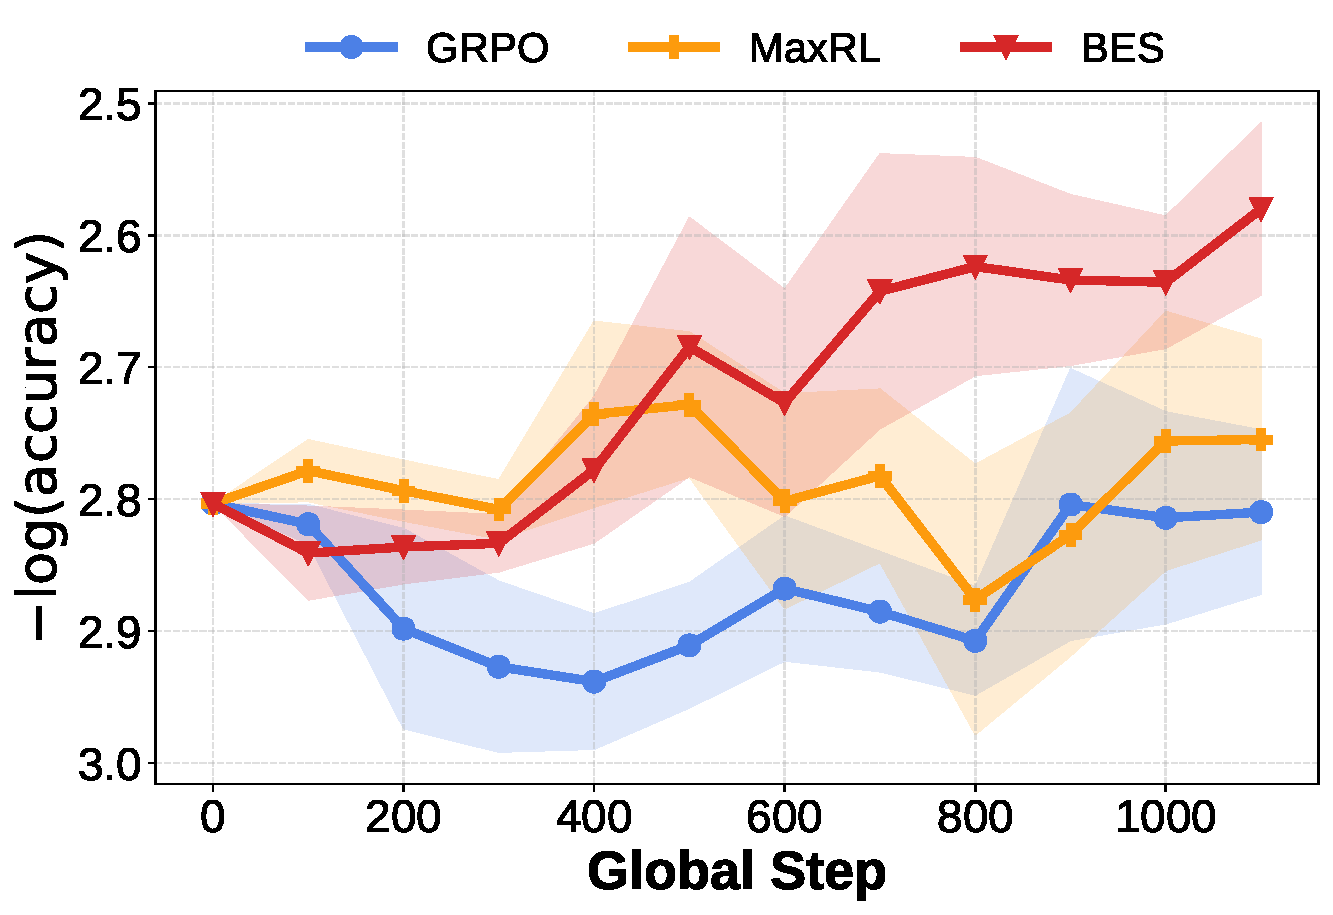
\includegraphics[width=0.43\textwidth]{images/bes_vs_baselines_overall.pdf}
\caption{EMA-smoothed validation accuracy on logical reasoning (Knights-and-Knaves).}
\label{fig:kk}
\vspace{-1em}

\end{figure}

\textbf{Baselines.} We select two post-training algorithms, GRPO~\citep{dsr1} and MaxRL~\citep{maxrl}, as baselines, as we apply \ours\ on top of MaxRL. We note that \ours\ is a sampling algorithm that is agnostic to the training method and can be applied on top of any post-training algorithm. 

\textbf{Training Setup.} We use Gemma-3-1B-it~\citep{gemma3} as the base model. 
To adapt the model to the Knights-and-Knaves benchmark, we first perform a cold start by fine-tuning on 1K SFT examples generated using the official data generation pipeline for 3 epochs, followed by 4 epochs of post-training on 5K problems, during which we compare the different methods on a 1.3K validation set. Detailed experimental configurations are provided in Appendix~\ref{app:logical_setup}. 

\textbf{Results.} As shown in Figure~\ref{fig:kk}, due to the difficulty of the training set, GRPO and MaxRL show little to no improvement during training, while \ours\ steadily improves on the validation set throughout training, demonstrating that \ours\ is more effective at discovering high-quality training samples.

\subsubsection{Multi-Hop Reasoning}



\begin{table*}[b]
\centering
\renewcommand{\arraystretch}{1.20}
\vspace{-1em}
\vspace{6pt}
\resizebox{\textwidth}{!}{%
\begin{tabular}{@{} l cccc @{}}
\toprule
\textbf{Method} 
& \textbf{Accuracy (\%, $\uparrow$)} 
& \textbf{\# Valid Search ($\uparrow$)} 
& \textbf{\# Valid Actions ($\uparrow$)} 
& \textbf{Finish Ratio ($\uparrow$)} \\
\midrule
\multicolumn{5}{@{}l}{\textit{Llama-3.2-3B-Instruct}} \\
\midrule[\lightrulewidth]
\rowcolor{cellbase}  Base model & 4.0 & -- & -- & -- \\
\rowcolor{cellbase}   + GRPO & 2.1 (-1.9) & 0.84 & 0.20 & 0.64 \\
\rowcolor{cellbase}  + Tree-GRPO & 3.9 (-0.1) & 1.50 & 2.14 & 0.64 \\
\rowcolor{tabband}   + \ours & \textbf{7.0 (+3.0)} & \textbf{2.31} & \textbf{3.29} & \textbf{0.97} \\
\midrule
\multicolumn{5}{@{}l}{\textit{Llama-3.1-8B-Instruct}} \\
\midrule[\lightrulewidth]
\rowcolor{cellbase}  Base model & 6.6 & -- & -- & -- \\
\rowcolor{cellbase}   + GRPO & 5.6 (-1.0) & 1.46 & 1.83 & 0.37 \\
\rowcolor{cellbase}  + Tree-GRPO & 7.4 (+0.8) & 0.65 & 1.36 & 0.71 \\
\rowcolor{tabband}   + \ours & \textbf{10.4 (+3.8)} & \textbf{2.11} & \textbf{3.05} & \textbf{0.94} \\
\bottomrule
\end{tabular}%
}
\label{tab:multihop}
\caption{Multi-hop reasoning post-training results on
MuSiQue with Llama-3.2-3B-Instruct and
Llama-3.1-8B-Instruct. We report accuracy, number of
valid searches, number of valid actions, and finish ratio. Higher is
better for all metrics. \textbf{Bold} denotes the best performing
method per backbone.}
\end{table*}

For multi-hop reasoning, we use the MuSiQue dataset~\citep{musique}. In this task, the agent must answer complex questions that require retrieving and integrating information across multiple documents, where no single document contains the complete answer. 

\textbf{Baselines.} We compare against GRPO~\citep{dsr1} and Tree-GRPO~\citep{treegrpo}, with the latter being the current state-of-the-art method for search agent post-training. We apply \ours\ on top of GRPO.

\textbf{Training Setup.} We adopt the training setup of Tree-GRPO~\citep{treegrpo}, using Llama-3.2-3B-Instruct and Llama-3.1-8B-Instruct~\citep{llama3} as base models. During the search process, the agent can perform multiple search actions before producing a final answer. Search results are provided by an offline Wikipedia server. We use the 3--4 hop solvable subset of the MuSiQue training set as our training data and train for 2 epochs, as additional epochs lead to training collapse. We evaluate on the full official MuSiQue validation set. Detailed configurations are provided in Appendix~\ref{app:qa_setup}.

\textbf{Results.} As shown in Table~\ref{tab:multihop}, GRPO consistently degrades from the base model on both scales, likely due to reward hacking where the model learns to skip search actions and guess directly, as reflected by its low number of valid searches. Tree-GRPO provides marginal improvement on the 8B model ($+0.8\%$) but fails to improve the 3B model. In contrast, \ours\ achieves substantial gains on both scales ($+3.0\%$ on 3B, $+3.8\%$ on 8B), outperforming all baselines by a wide margin. Beyond accuracy, \ours\ also produces agents with significantly more valid search actions and higher finish ratios, indicating that the trained agents learn to actively search rather than randomly guessing.



\subsection{Bidirectional Evolutionary Search for Inference}
At inference time, we evaluate the ability of \ours\ to solve open problems. Specifically, we consider three benchmarks: Circle Packing (Square), which seeks to pack $N$ circles into a unit square with maximum radius; Circle Packing (Rect), the analogous problem for a rectangular container; and Heilbronn (Convex), which seeks to place $N$ points in the unit square to maximize the minimum area of any convex polygon formed by subsets of the points.

\begin{table*}[h]
\centering
\vspace{-1em}
\renewcommand{\arraystretch}{1.20}
\vspace{6pt}
\resizebox{\textwidth}{!}{%
\begin{tabular}{@{} l cc cc cc @{}}
\toprule
\multirow{2}{*}{\textbf{Strategy}}
& \multicolumn{2}{c}{\textbf{Circle Packing (Square)}} 
& \multicolumn{2}{c}{\textbf{Circle Packing (Rect.)}} 
& \multicolumn{2}{c}{\textbf{Heilbronn (Convex)}} \\
\cmidrule(lr){2-3}
\cmidrule(lr){4-5}
\cmidrule(lr){6-7}
& Avg. & Best 
& Avg. & Best 
& Avg. & Best \\
\midrule
\multicolumn{7}{@{}l}{\textit{Human \& High-compute closed-source framework}} \\
\midrule[\lightrulewidth]
\rowcolor{cellbase} Human & -- & 2.634 & -- & 2.364 & -- & 0.0306 \\
\rowcolor{cellbase}  AlphaEvolve & -- & 2.635 & -- & 2.3658 & -- & 0.0309 \\
\midrule
\multicolumn{7}{@{}l}{\textit{Open-source frameworks}} \\
\midrule[\lightrulewidth]
\rowcolor{cellbase} OpenEvolve & 2.531 $\pm$ .018 & 2.541 & 2.267 $\pm$ .014 & 2.276 & 0.025 $\pm$ .005 & \textbf{0.027} \\
\rowcolor{cellbase}  GEPA & 2.613 $\pm$ .022 & 2.628 & 2.326 $\pm$ .023 & 2.354 & 0.025 $\pm$ .002 & \textbf{0.027} \\
\midrule
\multicolumn{7}{@{}l}{\textit{Base framework}} \\
\midrule[\lightrulewidth]
\rowcolor{cellbase} ShinkaEvolve & 2.464 $\pm$ .083 & 2.541 & 2.335 $\pm$ .026 & 2.358 & 0.023 $\pm$ .005 & 0.026 \\
\midrule
\multicolumn{7}{@{}l}{\textit{Ours}} \\
\midrule[\lightrulewidth]
\rowcolor{tabband}  \ours & \textbf{2.623} $\pm$ .014 & \textbf{2.632} & \textbf{2.349} $\pm$ .012 & \textbf{2.360} & \textbf{0.026} $\pm$ .001 & \textbf{0.027} \\
\bottomrule
\end{tabular}%
}
\label{tab:ops}
\caption{Open problem solving benchmarks with GPT-5 as the
backbone model. We report \textbf{Mean $\pm$ Std} and \textbf{Best}
objective values ($\uparrow$). \textbf{Bold} denotes the best
performing method.}
\end{table*}

\textbf{Baselines.} We compare against three open-source frameworks: OpenEvolve~\citep{openevolve}, GEPA~\citep{gepa}, and ShinkaEvolve~\citep{shinkaevolve}.  All baseline results are taken from SkyDiscover~\citep{skydiscover}, which uses the same backbone model, compute budget, and configuration as ours.  We apply \ours\ on top of ShinkaEvolve. For reference, we also include the results of human experts and AlphaEvolve~\citep{alphaevolve}, which is closed-source and uses significantly more compute than all other frameworks.

\textbf{Setup.} ShinkaEvolve maintains a population of candidate programs and iteratively proposes modifications. Since directly concatenating model outputs is not meaningful on this benchmark (where candidates are executable programs), we implement the evolution operators by prompting LLMs. We use GPT-5 as the backbone model. Detailed configurations are provided in Appendix~\ref{app:inference_setup}. 

\textbf{Results.} As shown in Table~\ref{tab:ops}, \ours\ outperforms open-source frameworks on every benchmark.  Notably, \ours\ also exhibits much lower variance across runs than all baselines, indicating the search is more stable and reliable. In Appendix~\ref{app:program}, we list a summary of the best programs discovered by \ours.




\subsection{Ablation Study}
\begin{figure}[t]
\vspace{-1em}
\centering
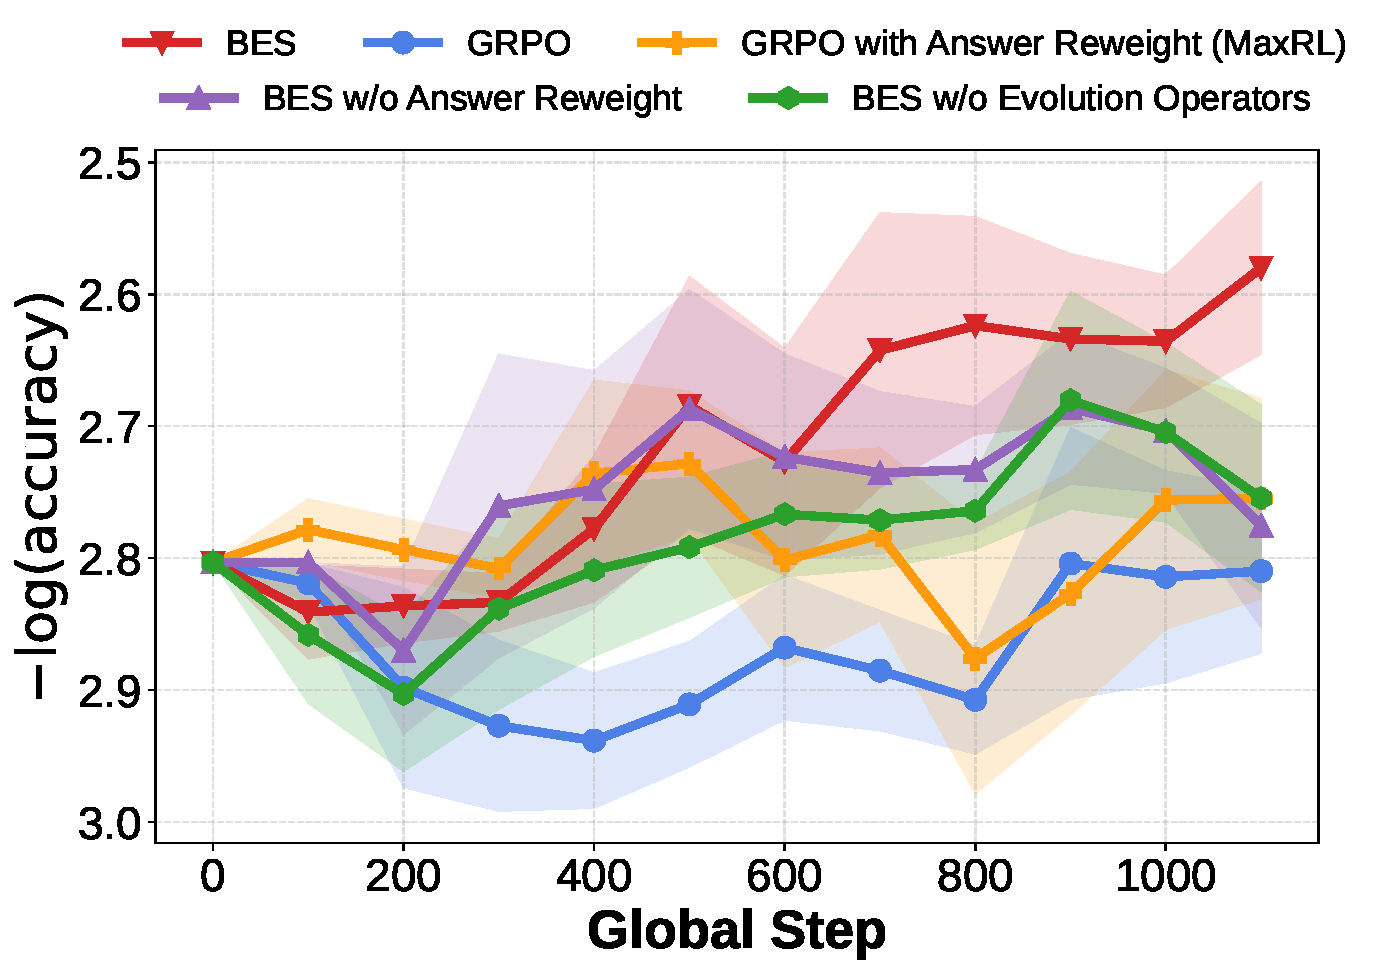
\includegraphics[width=0.43\textwidth]{images/bes_full_overall.pdf}
\vspace{-1em}
\caption{Ablation study on logical reasoning.}
\label{fig:kk_abl}
\vspace{-1em}

\end{figure}

We conduct an ablation study on the Knights-and-Knaves benchmark. On this benchmark, \ours\ combines bidirectional evolutionary search for discovering high-quality samples with MaxRL's answer reweighting for training. We therefore consider two ablations: (1) removing answer reweighting; and (2) removing the evolution operators to verify that both bidirectional search and evolution operators are necessary. As shown in Figure~\ref{fig:kk_abl}, both ablations underperform the full \ours\ method, while still outperforming the GRPO and MaxRL baselines. This confirms the effectiveness of each component in our approach.


\subsection{Cost Analysis}

\textbf{Post-Training.} To evaluate the cost-effectiveness of \ours, we compare the per-step wall-clock time and final accuracy across GRPO, Tree-GRPO, and \ours\ when training Llama-3.2-3B-Instruct on the agentic search task. We report the median wall-clock time per step throughout the training process.

\begin{table}[!htbp]
\centering
\renewcommand{\arraystretch}{1.20}
\begin{tabular}{lccc}
\toprule
\textbf{Method} & \textbf{Accuracy (\%)} & \textbf{\# Valid Search} & \textbf{Walltime (s)} \\
\midrule
\rowcolor{cellbase} GRPO & 2.1 (-1.9) & 0.84 & 64 \\
\rowcolor{cellbase}  Tree-GRPO & 3.9 (-0.1) & 1.50 & 240 \\
\rowcolor{tabband} \ours & \textbf{7.0 (+3.0)} & \textbf{2.31} & 309 \\
\bottomrule
\end{tabular}
\label{tab:cost_posttraining}
\caption{Cost analysis for multi-hop reasoning post-training on Llama-3.2-3B-Instruct.}
\end{table}

Notably, the low wall-clock time of GRPO is misleading: during training, GRPO quickly exhibits reward hacking, with the model learning to skip search actions and guess answers directly, as reflected by its low number of valid searches. In contrast, \ours\ incurs less than 30\% additional overhead compared to Tree-GRPO, while achieving significantly better performance across all metrics.

\textbf{Inference.} We compare the API cost of \ours\ against ShinkaEvolve across all three open problem solving benchmarks. As shown in Table~\ref{tab:cost_inference}, \ours\ achieves consistently higher average values while incurring modest additional API costs.

\vspace{-0.5em}
\begin{table}[!htbp]
\centering
\renewcommand{\arraystretch}{1.15}
\begin{tabular}{lccccccccc}
\toprule
& \multicolumn{3}{c}{\textbf{Circle Packing (Sq.)}} & \multicolumn{3}{c}{\textbf{Circle Packing (Rect.)}} & \multicolumn{3}{c}{\textbf{Heilbronn (Convex)}} \\
\cmidrule(lr){2-4} \cmidrule(lr){5-7} \cmidrule(lr){8-10}
\textbf{Method} & Avg. & Best & Cost & Avg. & Best & Cost & Avg. & Best & Cost \\
\midrule
\rowcolor{cellbase} ShinkaEvolve & 2.464 & 2.541 & \$13.0 & 2.335 & 2.358 & \$11.9 & 0.023 & 0.026 & \$11.5 \\
\rowcolor{tabband} \ours & \textbf{2.623} & \textbf{2.632} & \$18.6 & \textbf{2.349} & \textbf{2.360} & \$14.0 & \textbf{0.026} & \textbf{0.027} & \$13.7 \\
\bottomrule
\end{tabular}
\label{tab:cost_inference}
\caption{Cost analysis for open problem solving. We report average API cost per generation.}
\end{table}
\vspace{-1em}

\section{Related Work}

\textbf{Self-Improvement for LLM and Agent.} A growing line of work studies how language models and agents can improve using their own outputs to self-evolve~\citep{selfimprovement, selftraining}. STaR~\citep{star} bootstraps reasoning by filtering correct rationales for fine-tuning, while Self-Refine~\citep{madaan2023self} revises outputs at inference time through self-generated feedback. Self-Rewarding Language Models~\citep{selfreward} use the model itself as a judge for preference optimization. In agentic settings, Reflexion~\citep{shinn2023reflexion} converts environmental feedback into verbal reflections, and Voyager~\citep{wang2023voyager} accumulates reusable skills through continual exploration. These methods typically refine individual trajectories or rely on the model to judge its own outputs. In contrast, \ours\ treats self-improvement as a structured search problem, systematically discovering high-quality solutions that facilitate model self-improvement.

\textbf{Search in LLM and Agent.} Recent work applies search to both training and inference of LLMs and agents~\citep{efficientevolution, funsearch}. On the training side, tree-structured exploration provides richer supervision and finer-grained credit assignment than standard rollout-based methods. Tree-GRPO~\citep{treegrpo} and TreeRL~\citep{treerl} integrate tree search directly into reinforcement learning, while ReST-MCTS*~\citep{restmcts}, MCTS-DPO~\citep{mctsdpo}, and rStar-Math~\citep{rstarmath} use search to bootstrap higher-quality training data for self-improvement. On the inference side, Tree of Thoughts~\citep{tot}, Graph of Thoughts~\citep{got}, and RAP~\citep{rap} established reasoning as an explicit search problem by expanding chain-of-thought into tree-structured exploration~\citep{abmcts}. More recently, evolutionary approaches such as AlphaEvolve~\citep{alphaevolve}, ShinkaEvolve~\citep{shinkaevolve}, and ThetaEvolve~\citep{thetaevolve} tackle hard and even open problems~\citep{languageevolutionary} by maintaining candidate populations with LLM-driven mutations and external evaluation. However, these methods predominantly rely on tree search and thus struggle to explore beyond the policy's own distribution.

\textbf{Classical Search Methods.} The recent surge of search-based methods in LLMs and agents draws on a long history of classical search. In symbolic planning and graph search, algorithms such as A*~\citep{astar} and bidirectional search introduced core principles including heuristic guidance, frontier expansion, and search-space reduction. Branch-and-bound methods~\citep{bbsurvey}, which prune subtrees whose bounds certify suboptimality, offer a natural analogy for modern methods that use verifiers to discard unpromising candidates early. Evolutionary methods, including genetic search~\citep{genesearch,geneprogram} and differential evolution~\citep{differentialevolution}, optimize by maintaining and iteratively refining candidate populations. 
\section{Conclusion}

In this paper, we present \ours, a bidirectional evolutionary search framework that addresses two fundamental limitations of existing search methods for LLMs and agents: sparse verification signals and confined candidate generation. \ours\ couples forward search, which evolves candidates through expansion and four evolution operators, with backward search, which recursively decomposes problems into verifiable sub-goals to provide dense intermediate feedback. We provide theoretical justification showing that candidates generated by expansion-only search are confined to a narrow entropy shell while evolution operators can escape it, and that backward sub-goal decomposition exponentially reduces the number of candidates needed to find a solution. Experiments on logical reasoning, multi-hop reasoning, and open problem solving demonstrate that \ours\ consistently improves over strong baselines in both post-training and inference settings. We hope that \ours\ provides useful insights for self-improving language models and agents.

% 
\bibliography{ref}
\bibliographystyle{plainnat}


\appendix

\etocdepthtag.toc{appendix}
\etocsettocstyle{\section*{Appendix - Table of Contents}}{}
\tableofcontents
\vspace{1em}


\section{Pseudo Code}
\label{app:algo}

We provide the full pseudocode for \ours\ below. Algorithm~\ref{alg:bes} describes the main loop, which alternates between forward search steps (Algorithm~\ref{alg:forward}) and backward scoring (Algorithm~\ref{alg:backward}). Every $K_{\mathrm{dec}}$ steps, the backward goal tree is refined by decomposing an unsolved leaf into finer sub-goals (Algorithm~\ref{alg:decompose}), after which all pool scores are recomputed under the updated tree.

\begin{algorithm}[h]
\caption{\ours: Bidirectional Evolutionary Search}
\label{alg:bes}
\begin{algorithmic}[1]
\Require problem $x$, policy $\pi_\theta$, verifier $V$, budget $B$, decomposition interval $K_{\mathrm{dec}}$
\State Initialize $\mathcal{G}$ with root goal $g_0$; prompt $\pi_\theta$ to decompose $g_0$ into initial sub-goals
\State $\mathcal{P} \leftarrow \{n_0\}$ with $n_0 = ()$ \Comment{Empty root node}
\For{$t = 0, 1, \ldots$ \textbf{while} $\mathrm{calls}(t) < B$}
    \State $n' \leftarrow \textsc{ForwardStep}(\mathcal{P}, \mathcal{C}_t, \mathcal{G}, \tau_t)$ \Comment{Algorithm~\ref{alg:forward}}
    \State $s(n') \leftarrow \textsc{BackwardScore}(n', g_0, \mathcal{G})$ \Comment{Algorithm~\ref{alg:backward}}
    \State $\mathcal{P} \leftarrow \mathcal{P} \cup \{n'\}$
    \If{$(t+1) \bmod K_{\mathrm{dec}} = 0$}
        \State $\mathcal{G} \leftarrow \textsc{BackwardDecompose}(x, \mathcal{G}, \mathcal{P})$ \Comment{Algorithm~\ref{alg:decompose}}
        \For{$n \in \mathcal{P}$} \Comment{Recompute all scores under refined tree}
            \State $s(n) \leftarrow \textsc{BackwardScore}(n, g_0, \mathcal{G})$
        \EndFor
    \EndIf
    \If{$n'$ is terminal $\wedge$ $V(x, n') = 1$}
        \State \Return $n'$
    \EndIf
\EndFor
\State \Return $\arg\max_{n \in \mathcal{P}:\, \mathrm{terminal}(n)} V(x, n)$
\end{algorithmic}
\end{algorithm}

Algorithm~\ref{alg:forward} details a single forward search step. An operator is sampled from the fixed distribution over the five operators. Single-parent operators (expansion and deletion) select a parent via Boltzmann selection based on backward scores; two-parent operators (combination, translocation, crossover) select a pair that maximizes joint sub-goal coverage.

\begin{algorithm}[h]
\caption{\textsc{ForwardStep}: Forward Search Step}
\label{alg:forward}
\begin{algorithmic}[1]
\Require pool $\mathcal{P}$, eligible set $\mathcal{C}_t$, goal tree $\mathcal{G}$, temperature $\tau_t$
\State Sample operator $o \in \{\textit{expand}, \textit{combine}, \textit{delete}, \textit{translocate}, \textit{crossover}\}$ with fixed probabilities
\If{$o \in \{\textit{expand}, \textit{delete}\}$} \Comment{Single-parent operators}
    \State Sample parent $n$ from $\mathcal{C}_t$ via Boltzmann selection (Eq.~\ref{eq:boltz})
    \If{$o = \textit{expand}$}
        \State Sample $K \sim \mathrm{Uniform}\{1, \ldots, K_{\max}\}$
        \State $n' \leftarrow (y_1, \ldots, y_t, y_{t+1}, \ldots, y_{t+K})$ where $y_{t+k} \sim \pi_\theta(\cdot \mid x \oplus y_{1:t+k-1})$
    \Else
        \State Sample $\ell \sim \mathrm{Uniform}\{2, \ldots, t-1\}$; \, $n' \leftarrow (y_1, \ldots, y_{\ell-1}, y_{\ell+1}, \ldots, y_t)$
    \EndIf
\Else \Comment{Two-parent operators}
    \State Sample pair $(n_a, n_b)$ from $\mathcal{C}_t$ via pair Boltzmann selection (Eq.~\ref{eq:bi_boltz})
    \State Compute shared prefix length $s$ and suffixes $\sigma_a, \sigma_b$
    \If{$o = \textit{combine}$}
        \State $n' \leftarrow y_{a,1:s} \oplus \sigma_a \oplus \sigma_b$
    \ElsIf{$o = \textit{translocate}$}
        \State Sample $r, q$; \, $n' \leftarrow y_{a,1:s} \oplus \sigma_a[1:r\!-\!1] \oplus (\sigma_b)_q \oplus \sigma_a[r\!+\!1:m_a]$
    \ElsIf{$o = \textit{crossover}$}
        \State Sample $i, j$; \, $n' \leftarrow y_{a,1:s} \oplus \sigma_a[1:i] \oplus \sigma_b[j\!+\!1:m_b]$
    \EndIf
\EndIf
\State \Return $n'$
\end{algorithmic}
\end{algorithm}

Algorithm~\ref{alg:backward} computes the backward score for a candidate node by recursively traversing the sub-goal tree. If a sub-goal is fully satisfied, the score is 1; otherwise, the score blends the local verifier output with the average score over its children.

\begin{algorithm}[h]
\caption{\textsc{BackwardScore}: Backward Search Scoring}
\label{alg:backward}
\begin{algorithmic}[1]
\Require candidate node $n$, sub-goal $g$, goal tree $\mathcal{G}$
\If{$V_g(x, n) = 1$}
    \State \Return $1$
\ElsIf{$\mathrm{ch}(g) \neq \emptyset$}
    \State \Return $\alpha \cdot V_g(x, n) + (1 - \alpha) \cdot \frac{1}{|\mathrm{ch}(g)|} \sum_{g' \in \mathrm{ch}(g)} \textsc{BackwardScore}(n, g', \mathcal{G})$
\Else
    \State \Return $V_g(x, n)$
\EndIf
\end{algorithmic}
\end{algorithm}

Algorithm~\ref{alg:decompose} refines the goal tree by selecting a random unsolved leaf sub-goal and prompting the policy to decompose it into finer children, each equipped with its own local verifier.

\begin{algorithm}[h]
\caption{\textsc{BackwardDecompose}: Goal Tree Decomposition}
\label{alg:decompose}
\begin{algorithmic}[1]
\Require problem $x$, current goal tree $\mathcal{G}$, pool $\mathcal{P}$
\State $\mathcal{L} \leftarrow \{g \in \mathcal{G} : \mathrm{ch}(g) = \emptyset \wedge \max_{n \in \mathcal{P}} V_g(x, n) < 1\}$ \Comment{Unsolved leaves}
\State Sample $g^*$ uniformly from $\mathcal{L}$
\State Prompt $\pi_\theta$ to decompose $g^*$ into children $\{g'_1, \ldots, g'_c\}$ with local verifiers $\{V_{g'_1}, \ldots, V_{g'_c}\}$
\State $\mathrm{ch}(g^*) \leftarrow \{g'_1, \ldots, g'_c\}$; \, add to $\mathcal{G}$
\State \Return $\mathcal{G}$
\end{algorithmic}
\end{algorithm}

\section{Formal Definitions of Evolution Operators}
\label{app:operators}

For two parents $n_a, n_b$, let $s=\max\{\ell:y_{a,1:\ell}=y_{b,1:\ell}\}$ denote their common-prefix length, and let $\sigma_a=(y_{a,s+1},\dots,y_{a,t_a})$ and $\sigma_b=(y_{b,s+1},\dots,y_{b,t_b})$ be their respective suffixes.

\textit{(i) Combination.} $n' = y_{a,1:s}\,\oplus\,\sigma_a\,\oplus\,\sigma_b$.

\textit{(ii) Deletion.} $n' = (y_{1},\dots,y_{\ell-1},\,y_{\ell+1},\dots,y_{t})$, where $\ell\sim\mathrm{Uniform}\{2,\dots,t-1\}$.

\textit{(iii) Translocation.} $n' = y_{a,1:s}\,\oplus\,\sigma_a[1:r-1]\,\oplus\,(\sigma_b)_q\,\oplus\,\sigma_a[r+1:m_a]$, where $r\sim\mathrm{Uniform}\{1,\dots,m_a\}$ and $q\sim\mathrm{Uniform}\{1,\dots,m_b\}$.

\textit{(iv) Crossover.} $n' = y_{a,1:s}\,\oplus\,\sigma_a[1:i]\,\oplus\,\sigma_b[j+1:m_b]$, where $i\in\{0,\dots,m_a\}$ and $j\in\{0,\dots,m_b-1\}$ are sampled uniformly.

\section{Theoretical Motivations}
\label{app:theory}


\subsection{Theoretical Motivation for Evolution Operators}
\label{app:theory-mutation}

In this section, we give a theoretical justification for the evolution operators. Expansion-only search builds candidates one lineage at a time. Evolution, by contrast, recombines blocks from different trajectories, so the number of reachable candidates grows as a Cartesian product of the per-block libraries.

Fix a task $x$ and a step horizon $T$. A trajectory is $Y=(y_1,\ldots,y_T)$, where each $y_t$ is a step:
\begin{equation}
  P(Y) := \pi_\theta(Y\mid x)
  =\prod_{t=1}^{T}P(y_t\mid y_{<t}).
\end{equation}

To quantify the uncertainty at each step, we introduce the \emph{surprisal} (pointwise information content) of the $t$-th step and its expected value, the \emph{conditional entropy}:
\begin{equation}
  Z_t := -\log P(Y_t \mid Y_{<t}),
  \qquad
  h_t(y_{<t}) := H_P(Y_t \mid Y_{<t} = y_{<t}).
\end{equation}
Intuitively, $Z_t$ measures how surprising the generated step is, while $h_t$ measures how uncertain the policy is about the next step on average, given the history so far.

Summing the per-step surprisals yields the total information content of the trajectory:
\begin{equation}
  S_T := -\log P(Y) = \sum_{t=1}^{T} Z_t.
\end{equation}
Taking its expectation recovers the trajectory-level entropy, which decomposes by the chain rule as
\begin{equation}
  H_T := H_P(Y) = \mathbb{E}_P[S_T]
  = \sum_{t=1}^{T} \mathbb{E}_P\bigl[h_t(Y_{<t})\bigr].
\end{equation}

Finally, let $\mathcal{F}_t = \sigma(Y_1,\dots,Y_t)$ denote the natural filtration, i.e.\ the information available after observing the first $t$ steps. This filtration will serve as the basis for the martingale analysis that follows.

% We make three assumptions on the policy.

% \begin{assumption}[Bounded per-step surprise]
% \label{assump:bounded}
% There exists $L<\infty$ such that for every reachable prefix and every step with positive probability, $-\log P(v\mid y_{<t})\le L$.
% \end{assumption}

% \begin{assumption}[Decaying step dependence]
% \label{assump:decay}
% There exists a summable nonnegative sequence $(\beta_\ell)_{\ell\ge1}$ with $C_\beta:=\sum_{\ell\ge1}\beta_\ell<\infty$ such that for every $s<t$, every prefix $y_{<s}$, and every two possible step values $v,v'$ at position $s$,
% \begin{equation}
% \left|
% \mathbb{E}\!\big[h_t(Y_{<t})\mid Y_{<s}=y_{<s},Y_s=v\big]
% -
% \mathbb{E}\!\big[h_t(Y_{<t})\mid Y_{<s}=y_{<s},Y_s=v'\big]
% \right|
% \le \beta_{t-s}.
% \end{equation}
% \end{assumption}

% \begin{assumption}[Linear block total correlation]
% \label{assump:tc}
% Partition the trajectory into $k \geq 2$ contiguous blocks $U_1, \ldots, U_k$ at fixed boundaries $0 = s_0 < s_1 < \cdots < s_k = T$. The block total correlation grows linearly in the horizon:
% \begin{equation}
%   \mathrm{TC}_P(U_1, \ldots, U_k) := \sum_{j=1}^k H_P(U_j) - H_P(U_1, \ldots, U_k) \;\geq\; \gamma T
% \end{equation}
% for some constant $\gamma > 0$.
% \end{assumption}

We assume that evolution operators and verification are computationally cheap relative to policy calls. This is typical in practice: evolution operators act by directly editing step sequences (Section~\ref{sec:forward}), and verification is fast for most tasks of interest, e.g.\ test-case execution for coding. The computational bottleneck is therefore mainly the number of policy calls. Other assumptions have been stated in Section~\ref{sec:theory-mutation}.

\subsubsection{Discussion of Assumptions}
\label{app:assumptions}

To begin with, we first briefly discuss why Assumptions~\ref{assump:bounded}--\ref{assump:tc} are mild and naturally satisfied in practice.

\paragraph{Assumption~\ref{assump:bounded} (bounded per-step surprise).} This requires that no single step carries unbounded information. It holds for any policy with a finite action space, which includes all LLMs with a fixed vocabulary and all agents with a discrete action set. For an LLM with vocabulary size $|\mathcal{V}|$, we have $L = \log |\mathcal{V}|$.

\paragraph{Assumption~\ref{assump:decay} (decaying step dependence).} This requires that changing a single step has diminishing influence on the conditional entropy of distant future steps. In practice, this is satisfied when the policy's effective context dependence decays with distance, a property that holds for finite-context models and, empirically, for transformer-based LLMs whose attention weights concentrate on recent tokens for most layers. For a policy with finite memory (e.g., a Markov chain of order $d$), $\beta_\ell = 0$ for all $\ell > d$, trivially satisfying the assumption.

\paragraph{Assumption~\ref{assump:tc} (linear block total correlation).} By the chain rule, the total correlation decomposes as $\mathrm{TC}_P = \sum_{j=1}^k I_P(U_j; U_{<j})$, where $I_P(U_j; U_{<j})$ is the mutual information between block $j$ and all preceding blocks. This term is strictly positive whenever block $j$ depends on its context, which is the generic case for coherent sequential reasoning: the content of later reasoning steps is informed by earlier ones. As long as each block's dependence on the past contributes at least a constant amount of mutual information, the total correlation grows linearly in the number of blocks, and hence linearly in $T$ when blocks have bounded size. Empirically, this is a weak requirement: even simple autoregressive models on natural language exhibit strong inter-block dependence, and reasoning traces exhibit even stronger dependence since later steps logically build on earlier conclusions.

\subsubsection{Shell Confinement of Expansion}

The deviation $S_T - H_T$ between a trajectory's actual information content and the expected entropy governs how tightly ordinary rollouts cluster around the typical set. We aim to show that this deviation is small with high probability. To this end, we decompose it into two terms and bound each separately.

\begin{lemma}[Martingale decomposition]
\label{lem:decomp}
Define
\begin{equation}
  D_t:=Z_t-h_t(Y_{<t}),
  \qquad
  M_T:=\sum_{t=1}^{T}D_t,
  \qquad
  R_T:=\sum_{t=1}^{T}\big(h_t(Y_{<t})-\mathbb{E}h_t(Y_{<t})\big).
\end{equation}
Then $(D_t,\mathcal{F}_t)$ is a martingale difference sequence, $|D_t|\le L$, and
\begin{equation}
  S_T-H_T=M_T+R_T.
  \label{eq:martingale-decomp}
\end{equation}
Here $M_T$ captures the per-step noise, while $R_T$ captures how the realized trajectory shifts the conditional entropy away from its unconditional mean.
\end{lemma}

\begin{proof}
By definition,
$\mathbb{E}[Z_t\mid \mathcal{F}_{t-1}] = H_P(Y_t\mid Y_{<t}) = h_t(Y_{<t})$,
so $\mathbb{E}[D_t\mid\mathcal{F}_{t-1}]=0$. Assumption~\ref{assump:bounded} gives $0\le Z_t\le L$. Since $h_t(Y_{<t})$ is the conditional expectation of $Z_t$, we also have $0\le h_t(Y_{<t})\le L$, hence $|D_t|\le L$. Finally, $S_T=\sum_t D_t + \sum_t h_t(Y_{<t})$ and $H_T=\sum_t\mathbb{E}h_t(Y_{<t})$, which proves Eq.~\eqref{eq:martingale-decomp}.
\end{proof}

\begin{lemma}[Concentration of $R_T$]
\label{lem:rt}
Under Assumption~\ref{assump:decay}, for every $u>0$,
\begin{equation}
  \Pr(|R_T|\ge u)
  \le 2\exp\!\left(-\frac{u^2}{2TC_\beta^2}\right).
  \label{eq:rt-bound}
\end{equation}
\end{lemma}

\begin{proof}
Let $G(Y)=\sum_{t=1}^{T}h_t(Y_{<t})$, so $R_T=G(Y)-\mathbb{E}G(Y)$. We construct a Doob martingale by progressively revealing the trajectory one step at a time. Define
\begin{equation}
  A_s=\mathbb{E}[G(Y)\mid Y_1,\dots,Y_s]
  = \sum_{t=1}^{s} h_t(Y_{<t}) + \sum_{t=s+1}^{T} \mathbb{E}[h_t(Y_{<t})\mid Y_1,\dots,Y_s],
\end{equation}
where the first sum is already determined by the observed steps, and the second sum averages over the unobserved future. Note that $A_0 = \mathbb{E}[G(Y)]$ and $A_T = G(Y)$, so $R_T = A_T - A_0 = \sum_{s=1}^{T}\delta_s$ where $\delta_s = A_s - A_{s-1}$.

Expanding the increment gives
\begin{equation}
  \delta_s = \sum_{t=s+1}^{T}\Big(\mathbb{E}[h_t(Y_{<t})\mid Y_1,\dots,Y_s] - \mathbb{E}[h_t(Y_{<t})\mid Y_1,\dots,Y_{s-1}]\Big).
\end{equation}
Each term measures how much the prediction of $h_t$ changes upon revealing $Y_s$. By Assumption~\ref{assump:decay}, this change is bounded by $\beta_{t-s}$ for each $t>s$. Therefore
\begin{equation}
  |\delta_s|\le \sum_{t=s+1}^{T}\beta_{t-s}\le \sum_{\ell=1}^{\infty}\beta_\ell = C_\beta.
\end{equation}
Since $(A_s)$ is a martingale, $\mathbb{E}[\delta_s\mid Y_1,\dots,Y_{s-1}]=0$. Applying the Azuma-Hoeffding inequality to $R_T=\sum_{s=1}^{T}\delta_s$ with bounded increments $|\delta_s|\le C_\beta$ gives Eq.~\eqref{eq:rt-bound}.
\end{proof}

\begin{lemma}[Concentration of $M_T$]
\label{lem:mt}
The first term $M_T$ is itself a martingale with bounded increments $|D_t| \le L$. Let
\begin{equation}
  V_T:=\sum_{t=1}^{T}\mathbb{E}[D_t^2\mid\mathcal{F}_{t-1}].
\end{equation}
If $V_T\le v_T$ almost surely for a deterministic $v_T$, then for every $u>0$,
\begin{equation}
  \Pr(|M_T|\ge u)
  \le 2\exp\!\left(-\frac{u^2}{2(v_T+Lu/3)}\right).
  \label{eq:mt-freedman}
\end{equation}
\end{lemma}

\begin{proof}
This is Freedman's inequality for martingales with increments bounded by $L$, applied to $M_T$ and $-M_T$. If no sharper variance proxy is available, the worst-case bound $v_T=TL^2$ is valid.
\end{proof}


Combining the two concentration results yields a finite-sample analogue of the asymptotic equipartition property (AEP): with high probability, the information content of a trajectory is close to the expected entropy.

\begin{theorem}[Finite-sample AEP for policy rollouts]
\label{thm:aep}
Under Assumptions~\ref{assump:bounded}--\ref{assump:decay} and the variance condition in Lemma~\ref{lem:mt},
\begin{equation}
  \Pr(|S_T-H_T|\ge u)
  \le
  2\exp\!\left(-\frac{u^2}{8(v_T+Lu/6)}\right)
  +2\exp\!\left(-\frac{u^2}{8TC_\beta^2}\right).
  \label{eq:aep}
\end{equation}
In particular, if $v_T=O(T)$, then for every fixed $\epsilon>0$,
\begin{equation}
  \Pr\!\left(\left|\frac{S_T}{T}-\frac{H_T}{T}\right|\ge\epsilon\right)
  \le \exp(-\Omega(T)).
\end{equation}
\end{theorem}

\begin{proof}
By Lemma~\ref{lem:decomp}, $S_T-H_T=M_T+R_T$. A union bound gives
$\Pr(|S_T-H_T|\ge u) \le \Pr(|M_T|\ge u/2)+\Pr(|R_T|\ge u/2)$.
Applying Lemma~\ref{lem:mt} and Lemma~\ref{lem:rt} with threshold $u/2$ proves Eq.~\eqref{eq:aep}. Taking $u=\epsilon T$ and $v_T=O(T)$ gives the exponential concentration rate.
\end{proof}


\begin{corollary}[Shell confinement]
\label{cor:shell}
For $\epsilon>0$, define the typical set
\begin{equation}
  A_\epsilon^{(T)}:=\{y:|-\log P(y)-H_T|\le\epsilon T\}.
\end{equation}
Then $P(A_\epsilon^{(T)})\ge1-\exp(-\Omega(T))$ under Theorem~\ref{thm:aep}. Moreover,
\begin{equation}
  |A_\epsilon^{(T)}|\le\exp(H_T+\epsilon T).
  \label{eq:typical-upper}
\end{equation}
In other words, almost all rollouts land in a set of size $\approx \exp(H_T)$. Expansion-only search, regardless of how it selects prefixes, can only explore within this shell.
\end{corollary}

\begin{proof}
The probability statement follows from Theorem~\ref{thm:aep}. Every $y\in A_\epsilon^{(T)}$ satisfies $P(y)\ge\exp(-(H_T+\epsilon T))$, so summing probabilities gives $1\ge |A_\epsilon^{(T)}|\exp(-(H_T+\epsilon T))$, which proves Eq.~\eqref{eq:typical-upper}.
\end{proof}

\subsubsection{Shell Escape via Evolution}

We now show that evolution operators construct candidates whose expected log-probability falls strictly outside the entropy shell. We prove the results using crossover; the analysis for other evolution operators (combination, translocation) follows analogously.

\begin{lemma}[Splice-point KL identity]
\label{lem:splice}
Split a trajectory at position $s$ and write $V=Y_{1:s}$ and $U=Y_{s+1:T}$. Let $(V,U)$ and $(V',U')$ be two independent policy rollouts, and form the crossover trajectory $\widetilde{Y}=(V,U')$. The expected increase in native surprise is
\begin{equation}
  \mathbb{E}[-\log P(V,U')]-H_T
  =\mathbb{E}_{V,V'}
  \left[D_{\mathrm{KL}}(P_{U\mid V'}\|P_{U\mid V})\right].
  \label{eq:splice-kl}
\end{equation}
Equivalently,
\begin{equation}
  \mathbb{E}[-\log P(V,U')]-H_T
  =I_P(V;U)+D_{\mathrm{KL}}(P_V\otimes P_U\|P_{V,U})
  \ge I_P(V;U).
  \label{eq:splice-mi}
\end{equation}
The gap is strictly positive whenever the suffix distribution $P_{U\mid V}$ depends on the prefix.
\end{lemma}

\begin{proof}
Using $P(V,U)=P_V(V)P_{U\mid V}(U)$,
\begin{align}
  \mathbb{E}[-\log P(V,U')]
  &=H(V)+\mathbb{E}_{V,V'}\mathbb{E}_{U\sim P_{U\mid V'}}[-\log P_{U\mid V}(U)],\\
  H_T
  &=H(V)+\mathbb{E}_{V'}H(P_{U\mid V'}).
\end{align}
Subtracting gives Eq.~\eqref{eq:splice-kl}. The marginal law of $(V,U')$ is $P_V\otimes P_U$, so the same difference equals the cross-entropy gap $H(P_V\otimes P_U,P_{V,U})-H(P_{V,U})$, which is
$H(P_V\otimes P_U)+D_{\mathrm{KL}}(P_V\otimes P_U\|P_{V,U})-H(P_{V,U})$.
Since $H(P_V\otimes P_U)-H(P_{V,U})=I_P(V;U)$, Eq.~\eqref{eq:splice-mi} follows.
\end{proof}

Lemma~\ref{lem:splice} analyzes crossover at a single splice point. We now generalize to $k$-way block evolution, where a trajectory is partitioned into multiple blocks and each block is drawn from a different seed trajectory.

Fix a partition $0=s_0<s_1<\cdots<s_k=T$ and define blocks $U_j=Y_{s_{j-1}+1:s_j}$. Let $P$ denote the joint law of $(U_1,\ldots,U_k)$ under the policy, and let $P_j$ be the marginal law of $U_j$. A $k$-way blockwise evolution draws $k$ independent seed trajectories and takes block $j$ from seed $j$. The resulting distribution is
\begin{equation}
  Q=\bigotimes_{j=1}^{k}P_j.
  \label{eq:product-law}
\end{equation}

\begin{lemma}[Block evolution cross-entropy gap]
\label{lem:tc}
For $\widetilde{Y}\sim Q$,
\begin{equation}
  \mathbb{E}_{Q}[-\log P(\widetilde{Y})]-H(P)
  =\mathrm{TC}_P(U_1,\ldots,U_k)+D_{\mathrm{KL}}(Q\|P)
  \ge\mathrm{TC}_P(U_1,\ldots,U_k),
  \label{eq:tc-gap}
\end{equation}
where $\mathrm{TC}_P(U_1,\ldots,U_k) := \sum_{j=1}^{k}H_P(U_j)-H_P(U_1,\ldots,U_k)$ is the block total correlation.
\end{lemma}

\begin{proof}
The expected surprise of an evolution sample under the policy is the cross entropy $H(Q,P)=H(Q)+D_{\mathrm{KL}}(Q\|P)$. Since $Q$ is the product of the policy's block marginals, $H(Q)=\sum_j H_P(U_j)$. Subtracting $H(P)=H_P(U_1,\ldots,U_k)$ gives Eq.~\eqref{eq:tc-gap}.
\end{proof}


We can now state the main theorem.


\noindent\textbf{Theorem~\ref{thm:shell}} (Shell confinement and escape)\textbf{.}
\textit{Restated from Section~\ref{sec:theory-mutation}.}
\medskip

\noindent Under Assumptions~\ref{assump:bounded}--\ref{assump:tc}, define the typical set $A_\epsilon^{(T)}:=\{y:|-\log P(y)-H_T|\le\epsilon T\}$.

\textit{(a) Shell confinement.} Every trajectory $Y \sim P$ produced by expansion satisfies $\Pr[Y \notin A_\epsilon^{(T)}] \leq \exp(-\Omega(T))$. That is, expansion-only search is confined to a typical set of size at most $\exp(H_T + \epsilon T)$.

\textit{(b) Shell escape.} Let $Q = \bigotimes_{j=1}^k P_j$ be the $k$-way evolution distribution. For any $\epsilon < \gamma$,
\begin{equation*}
  \mathbb{E}_Q[-\log P(\widetilde{Y})] \;\geq\; H_T + \gamma T \;>\; H_T + \epsilon T,
\end{equation*}
so evolution candidates have expected log-probability strictly beyond the shell boundary. Moreover,
\begin{equation*}
  \Pr_Q\!\left[\widetilde{Y} \in A_\epsilon^{(T)}\right] \;\leq\; 1 - \frac{(\gamma - \epsilon)T}{LT - H_T - \epsilon T} \;<\; 1,
\end{equation*}
confirming that a positive fraction of evolution candidates escape the shell.


\begin{proof}
Part~(a) is Corollary~\ref{cor:shell}.

For part~(b), Lemma~\ref{lem:tc} gives $\mathbb{E}_Q[-\log P(\widetilde{Y})] = H_T + \mathrm{TC}_P + D_{\mathrm{KL}}(Q \| P) \geq H_T + \gamma T$ by Assumption~\ref{assump:tc}, proving Eq.~\eqref{eq:escape-expectation}.

For Eq.~\eqref{eq:escape-prob}, let $p = \Pr_Q[\widetilde{Y} \in A_\epsilon^{(T)}]$. By Assumption~\ref{assump:bounded}, $-\log P(\widetilde{Y}) \in [0, LT]$ always. If $\widetilde{Y} \in A_\epsilon^{(T)}$ then $-\log P(\widetilde{Y}) \leq H_T + \epsilon T$. Therefore
\begin{equation}
  H_T + \gamma T \;\leq\; \mathbb{E}_Q[-\log P(\widetilde{Y})] \;\leq\; (H_T + \epsilon T)\,p + LT\,(1 - p).
\end{equation}
Rearranging: $p \leq \frac{LT - H_T - \gamma T}{LT - H_T - \epsilon T} = 1 - \frac{(\gamma - \epsilon)T}{LT - H_T - \epsilon T}$, which is strictly less than $1$ whenever $\gamma > \epsilon$.
\end{proof}

\subsection{Theoretical Motivation for Bidirectional Search}
\label{app:theory-bidirectional}

\noindent\textbf{Theorem~\ref{thm:bidir}} (Exponential advantage from backward sub-goal signals)\textbf{.}
\textit{Restated from Section~\ref{sec:theory-bidirectional}.}
\medskip

\noindent Let $N$ candidates be sampled independently. Terminal-only search requires
$N_{\mathrm{term}} = \Omega\!\left(1 / \prod_{i=1}^m p_i\right)$
candidates to obtain constant success probability. By contrast, backward-guided bidirectional search requires only
$N_{\mathrm{bidir}} = O\!\left(p_{\min}^{-1}\log(m/\delta)\right)$,
where $p_{\min}=\min_i p_i$,
to collect evidence for all sub-goals with probability at least $1-\delta$. In the symmetric case $p_i=p$, the ratio is
$N_{\mathrm{term}} / N_{\mathrm{bidir}} = \Omega\!\left(p^{-(m-1)} / \log(m/\delta)\right)$,
which is exponential in the number of sub-goals $m$.

\begin{proof}
For a single candidate, terminal success requires all sub-goals:
\[
  \Pr[V(x,n)=1]
  \le
  \Pr\!\left[\bigcap_{i=1}^m \{C_i(n)=1\}\right]
  =
  \prod_{i=1}^m p_i.
\]
Therefore, after \(N\) independent candidates, the probability that a
terminal-only method observes a complete solution is at most
\[
  1-\left(1-\prod_{i=1}^m p_i\right)^N.
\]
To make this probability constant, one needs
\[
  N=\Omega\!\left(\frac{1}{\prod_{i=1}^m p_i}\right).
\]

Now consider backward verification. The pool contains evidence for all
sub-goals if, for every \(i\), at least one sampled candidate satisfies
\(C_i(n)=1\). This event has probability
\[
  \prod_{i=1}^m \left(1-(1-p_i)^N\right).
\]
Using \((1-p_i)^N\le e^{-Np_i}\), we obtain
\[
  \Pr[\text{some sub-goal is missing}]
  \le
  \sum_{i=1}^m e^{-Np_i}
  \le
  m e^{-N p_{\min}}.
\]
Thus
\[
  N\ge \frac{1}{p_{\min}}\log\frac{m}{\delta}
\]
ensures that the pool contains evidence for every sub-goal with probability at
least \(1-\delta\). Once such evidence exists, backward search identifies it
and evolution can recombine the corresponding partial trajectories. Hence
bidirectional search replaces the one-shot probability
\(\prod_i p_i\) by the much larger local probabilities \(p_i\), turning a
multiplicative hitting problem into a sub-goal collection problem. In the
symmetric case \(p_i=p\), terminal-only search needs
\(\Omega(p^{-m})\) candidates, whereas bidirectional search needs
\(O(p^{-1}\log(m/\delta))\), giving the stated exponential advantage.
\end{proof}

\section{Detailed Experimental Setup}
\label{app:setup}

\subsection{Logical Reasoning}
\label{app:logical_setup}

\paragraph{Resources.}
The trainer uses 2 H200 GPUs. A separate auxiliary GPU hosts a vLLM
server for the backward decomposer (a copy of Gemma-3-1B-it serving the
\textsc{Decompose} calls of the goal tree); the
trainer reaches it over HTTP.

\paragraph{Data.}
We generate the K\&K corpus with the official sampling pipeline. The SFT
cold-start corpus contains $1{,}000$ problems with $n_\mathrm{people}\in\{2,3,4\}$.
The post-training corpus contains $5{,}000$ problems with
$n_\mathrm{people}\in\{4,5,6\}$.
Validation contains $143$ problems per difficulty level
$n_\mathrm{people}\in\{2,\dots,10\}$ for a total of $1{,}287$ problems.

\paragraph{Training schedule.}
Stage~1 is a 3-epoch supervised fine-tuning on the SFT corpus to teach the
output format. Stage~2 is post-training. For \ours, each training step runs the forward-backward
search on every problem in the training batch, returning either eight
unique terminal trajectories (when the search hits the budget or finds
enough successes) or fewer, in which case the remaining slots are padded
with single-rollout samples to keep the GRPO group size fixed at $8$;
the trainer then conducts post-training on these samples. We compare against two baselines (GRPO and MaxRL),
both of which sample $8$ i.i.d.\ trajectories per problem.


\paragraph{Forward search.}
The forward search maintains a pool of partial reasoning trajectories
partitioned at paragraph granularity (\verb|\n\n|-separated reasoning
steps). At every search step we sample one of five actions:
\emph{combine} with probability $0.10$; \emph{deletion} with probability $0.05$; \emph{translocation} with probability $0.075$; \emph{crossover}
with probability $0.075$; and \emph{expansion}
with probability $0.70$.
The Boltzmann temperature $\tau$ is annealed linearly from
$\tau_0=2.0$ at step $0$ to $\tau_\mathrm{end}=1.0$ at step $B{-}2$.
A trajectory becomes \emph{terminal} when it contains a
``\verb|### Final Answer|'' marker followed by a parseable JSON map
\verb|{name: 0/1}|; the rule-based KK scorer then assigns reward
$r\in\{0,1\}$ from exact match against the ground-truth assignment. The
search runs until $B=200$ policy calls have been used or eight unique
terminal trajectories have been found.


\paragraph{Backward search.}
At the start of every \ours\ search on a puzzle we instantiate a goal
tree whose root goal is to identify every person's role correctly,
verified by the rule-based K\&K scorer applied to the trajectory's
final answer. The root expands into one sub-goal per person (determining whether that person is a knight or a knave) and each
per-person sub-goal further expands into elementary verification
strategies that human solvers commonly apply to K\&K puzzles, e.g.\
assume the opposite role and seek a contradiction, assume the correct
role and confirm consistency, or jointly fix two people's roles and
check pair-wise consistency. Leaf sub-goals are verified via
lightweight syntactic checks on the trajectory against the reasoning
markers each strategy is expected to produce.

Because Gemma-3-1B-it is too small to reliably perform open-ended goal
decomposition, we restrict the backward LLM's
role to scheduling traversal of this template tree rather than
constructing it. At the start of the search the decomposer is asked to
choose the order in which the per-person sub-goals should be verified;
every $D=10$ search steps thereafter it is asked to pick which
verification strategies should be activated under the next-in-line
per-person sub-goal. 
The recursive node score $s(n)$ is recomputed on every search step using $\alpha=0.3$.

\paragraph{Hyperparameters.}
Hyperparameters are listed in Table \ref{tab:hyperparams_logical}.

\begin{table*}[h]
\centering
\begin{tabularx}{\textwidth}{@{}lX@{}}
\toprule
\textbf{Category} & \textbf{Hyperparameter $=$ Value} \\
\midrule
\textbf{Model} &
backbone $=$ Gemma-3-1B-it; cold-start $=$ 3 epochs SFT on $1\,$K problems; \\
& post-training $=$ 4 epochs on $5\,$K problems. \\
\midrule
\textbf{Optimization} &
optimizer $=$ AdamW; learning\_rate $=$ $1\!\times\!10^{-6}$; \\
& train\_batch\_size $=$ 32; ppo\_mini\_batch\_size $=$ 32; \\
& ppo\_micro\_batch\_size\_per\_gpu $=$ 16; ppo\_epochs $=$ 1; \\
& clip\_ratio $=$ 0.2; grad\_clip $=$ 0.3; kl\_coef $=$ 0.0. \\
\midrule
\textbf{Generation} &
max\_prompt\_length $=$ 1024; max\_response\_length $=$ 4096; \\
& max\_model\_len $=$ 6144; train\_temperature $=$ 1.0; \\
& val\_temperature $=$ 0.6; val\_top\_p $=$ 0.95. \\
\midrule
\textbf{BES search} &
adv\_estimator $=$ \texttt{maxrl}; group\_size $=$ 8 trajectories/problem; \\
& search\_budget $=$ 200 policy calls/problem; \\
& decompose\_interval $=$ 10 search steps;  \\
\bottomrule
\end{tabularx}
\caption{Hyperparameters for the logical reasoning experiment (Knights-and-Knaves).}
\label{tab:hyperparams_logical}
\end{table*}


\subsection{Multi-Hop Reasoning}
\label{app:qa_setup}

\paragraph{Resources.}
The trainer uses 2 H200 GPUs. Two auxiliary
servers run independently and communicate with the trainer over HTTP:
(i) a retriever (E5 encoder + FAISS over the 2018 Wikipedia dump) on
1 H200 GPU, and (ii) a backward decomposition server hosting
Llama-3.1-8B-Instruct on 1 H200 GPU.

\paragraph{Data.}
We use the answerable subset of MuSiQue. The training set is the
3-to-4-hop solvable split of the MuSiQue training data and is held
fixed across methods; the validation set is the full official MuSiQue
validation set. 

\paragraph{Training schedule.}
Two epochs of post-training. At each
rollout the \ours\ search returns $8$ trajectories per problem; the same per-problem budget is used by the GRPO
and Tree-GRPO baselines for fair comparison. Two epochs are sufficient;
extra epochs lead to overfitting and training collapse.

\paragraph{Action format and reward.}
The agent emits actions as
\verb|<think>...</think>| followed by either \verb|<search>q</search>|
or \verb|<answer>...</answer>|. Each \verb|<search>| call goes to the offline
retriever which returns the top $3$ passages back to the agent inside
\verb|<information>...</information>| tokens. 


\paragraph{Forward search.}
The forward search maintains a candidate pool of trajectories per
question, where every trajectory is a sequence of
$(\langle\texttt{think}\rangle,\langle\texttt{search}\rangle,
\langle\texttt{information}\rangle)$ triples optionally followed by a
terminal $(\langle\texttt{think}\rangle,\langle\texttt{answer}\rangle)$
pair. Strict format validation is enforced on every expansion.

At every search step we sample one of five actions with the same
mixture used in the logical-reasoning experiment:
\emph{combination} $0.10$, \emph{deletion} $0.05$, \emph{translocation}
$0.075$, \emph{crossover} $0.075$, \emph{expansion} $0.70$. The evolution operators here operate at the triple boundary. The Boltzmann temperature $\tau$ is annealed linearly from
$\tau_0=1.5$ at step $0$ to $\tau_\mathrm{end}=0.3$ at the budget. We pick $\alpha=0.7$.


\paragraph{Backward search.}
Backward search decomposes each question into an ordered chain of atomic sub-questions. The
original question together with these sub-questions defines the
per-question goal tree.
The local verifier $V_{g_i}$ is queried by the forward search for
every candidate trajectory at every step, so a per-call LLM verifier would be impractical. We therefore
instantiate $V_{g_i}$ as a fast embedding model: every
$\langle\texttt{search}\rangle$ query that a trajectory $n$ has emitted
is embedded into the $\texttt{all-MiniLM-L6-v2}$ sentence-embedding
space, and the same is done for each sub-question. A sub-question
$g_i$ is declared \emph{covered} by trajectory $n$ when
\begin{equation}
\max_{q \in \mathrm{searches}(n)}\,
  \cos\bigl(\mathrm{emb}(q),\mathrm{emb}(g_i)\bigr) \;\ge\; \sigma_\mathrm{cov} = 0.6,
\end{equation}
i.e.\ when at least one of the trajectory's search queries
semantically aligns with the sub-question. 

Since a later sub-question's answer typically depends on those of the earlier ones, we evaluate sub-goals sequentially: a sub-goal is only checked if all preceding sub-goals have been satisfied.

\paragraph{Hyperparameters.}
Hyperparameters are listed in Table \ref{tab:hyperparams_multihop}.


\begin{table*}[h]
\centering
\begin{tabularx}{\textwidth}{@{}lX@{}}
\toprule
\textbf{Category} & \textbf{Hyperparameter $=$ Value} \\
\midrule
\textbf{Model} &
backbones $=$ \{Llama-3.2-3B-Instruct, Llama-3.1-8B-Instruct\}; \\
& post-training $=$ 2 epochs on the 3--4-hop solvable MuSiQue split. \\
\midrule
\textbf{Optimization} &
optimizer $=$ AdamW; learning\_rate $=$ $1\!\times\!10^{-6}$; \\
& lr\_warmup\_ratio $=$ 0.285; \\
& train\_batch\_size $=$ 128; val\_batch\_size $=$ 32; \\
& ppo\_mini\_batch\_size $=$ 16; ppo\_micro\_batch\_size $=$ 8; \\
& kl\_loss\_coef $=$ $1\!\times\!10^{-3}$; kl\_loss\_type $=$ low\_var\_kl. \\
\midrule
\textbf{Generation} &
max\_prompt\_length $=$ 4096; max\_response\_length $=$ 2048; \\
& max\_obs\_length $=$ 500; temperature $=$ 1.0; \\
&max\_turns $=$ 3. \\
\midrule
\textbf{BES search} &
adv\_estimator $=$ \texttt{grpo}; group\_size $=$ 8 trajectories/problem; \\
& search\_budget $=$ 50 policy calls/problem; $K$-parallel $=$ 4; \\
& embedder $=$ all-MiniLM-L6-v2; sim\_threshold\_$\sigma_\mathrm{cov}$ $=$ 0.6; \\
\midrule
\textbf{Retriever} &
encoder $=$ intfloat/e5-base-v2; index $=$ wiki-18 FAISS; topk $=$ 3. \\
\bottomrule
\end{tabularx}
\caption{Hyperparameters for the multi-hop reasoning experiment (MuSiQue).}
\label{tab:hyperparams_multihop}
\end{table*}


\subsection{Open Problem Solving}
\label{app:inference_setup}

\paragraph{Resources.}
All compute is on a single CPU node; LLM access is through the OpenAI
API. We use \texttt{gpt-5} with \texttt{reasoning\_effort = high} for
forward proposals, meta-reasoning, and backward decomposition. Each run
is capped at \$50 of API spend; baseline frameworks (OpenEvolve, GEPA,
ShinkaEvolve) are run under the same setting and we directly use the results from Skydiscover~\citep{skydiscover}.

\paragraph{Benchmarks.}
Three open optimization tasks: (i) \emph{Circle Packing (Square)}:
pack $n=26$ non-overlapping circles in the unit square to maximize the
sum of radii; (ii) \emph{Circle Packing (Rect)}: the same in a
fixed-aspect rectangle; (iii) \emph{Heilbronn (Convex, $n=13$)}: place
$13$ points in the unit square to maximize the minimum area of any
convex polygon formed by a subset of the points. We report mean and
best objective value across $3$ runs per benchmark.

\paragraph{Algorithm.}
We adopt ShinkaEvolve as the base program-evolution framework. A
population of executable Python programs is maintained in an islanded
SQLite archive; at each generation, parents are sampled from the
archive, mutated by an LLM-driven proposer, and the resulting offspring
are evaluated against the benchmark scorer. BES adds two components on
top: (a) the four evolution operators (combination, deletion, translocation,
crossover), realized as LLM-driven \emph{joint rewrites} of two parent
programs (since direct concatenation is not meaningful for executable
programs), and (b) a backward goal tree that supplies dense
intermediate scores.


\paragraph{Forward search.}

The four evolution operators of the main paper --- combination,
translocation, crossover, deletion --- are realized at the
program level. Direct token-level concatenation is not
meaningful for executable programs, so we pass both parents to the proposer with an operator-specific instruction (e.g.\ ``combine the
structural decisions of program A with the parameter choices of
program B'') and ask it to return a single new program implementing the requested edit. Detailed prompts are listed in Appendix \ref{app:prompts:forward}.

\paragraph{Backward search.}
In the backward goal tree, each leaf carries a Python verifier
expression that returns a continuous partial-progress score in
$[0,1]$, evaluated against a benchmark-supplied namespace describing the program's outputs. Detailed prompts are listed in Appendix \ref{app:prompts:backward}.

Tree growth is performed adaptively during the run. A decomposition pass is triggered whenever
the population has failed to improve on the raw objective for $S=5$
consecutive generations (improvement margin $\Delta=10^{-2}$): we
pick a leaf that no program in the archive has yet fully satisfied,
and ask the decomposer LLM  to
propose 2--4 child sub-goals that together cover the leaf, each with
its own natural-language description and Python verifier. This
adaptive schedule lets the tree grow into the kinds of bottlenecks the population actually encounters.

When calculating the score, in order not to hurt ground truth signals, we rank programs by a
\emph{bucket-interpolation} effective score: programs are first
bucketed by the raw objective at precision $10^{-2}$ and ranked by
bucket; within a bucket, the recursive backward score acts as an
intra-bucket sub-rank, scaled so that it can never push a program
past the next bucket boundary. This guarantees that any improvement
in the raw objective dominates any change in the backward signal, so
the backward score mainly acts as a tie-breaker among programs of similar raw scores.


\paragraph{Hyperparameters.}
Hyperparameters are listed in Table \ref{tab:hyperparams_inference}.

\begin{table*}[h]
\centering
\begin{tabularx}{\textwidth}{@{}lX@{}}
\toprule
\textbf{Category} & \textbf{Hyperparameter $=$ Value} \\
\midrule
\textbf{LLM} &
backbone $=$ gpt-5; reasoning\_effort $=$ high. \\
\midrule
\textbf{Evolution} &
num\_generations $=$ 100; max\_evaluation\_jobs $=$ 2; \\
& max\_proposal\_jobs $=$ 2; max\_db\_workers $=$ 2; \\
& max\_patch\_resamples $=$ 3; max\_patch\_attempts $=$ 2. \\
\midrule
\textbf{Operators} &
patch\_types $=$ \{diff, full, cross\} with probs $\{0.6, 0.3, 0.1\}$; \\
& BES operators $=$ \{combine, deletion, translocation, crossover\}. \\
\midrule
\textbf{Database} &
num\_islands $=$ 1; archive\_size $=$ 40; \\
& parent\_selection\_strategy $=$ weighted; parent\_selection\_lambda $=$ 10; \\
& effective\_score $=$ bucket-interpolation (precision $10^{-2}$). \\
\midrule
\textbf{BES backward} &
trigger $=$ stagnation; $S=5$ generations; margin $\Delta=10^{-2}$; \\
& children\_per\_decompose $=$ 2--4; max\_tree\_depth $=$ 2; \\
& recursive\_blend\_$\alpha$ $=$ 0.3; monotonic\_expansion $=$ True. \\
\bottomrule
\end{tabularx}
\caption{Hyperparameters for the open problem solving experiment.}
\label{tab:hyperparams_inference}
\end{table*}

\section{Case Study}
\label{app:case}

We illustrate the \ours\ search process on a multi-hop question answering example from the MuSiQue dataset. The question is: \textit{``What is the record label of the artist who originally recorded Back to Bedlam?''} The correct answer is Custard Records. Figure~\ref{fig:case} shows the full search trace.

\begin{figure}[!htbp]
\centering

\includegraphics[width=\linewidth]{images/demo.pdf}
\caption{Case study of \ours\ on a multi-hop reasoning problem. The forward search (top) explores two branches via expansion, both of which lead to wrong answers. A translocation operator then combines a reasoning step from the right branch into the left branch, producing a correct answer. The backward search (bottom) decomposes the original question into two sub-goals and provides dense verification feedback (green/red arrows) to guide parent selection.}
\label{fig:case}
\end{figure}

\paragraph{Backward search.} The backward search decomposes the original question into two sub-goals: (1) \textit{``Which artist originally recorded Back to Bedlam?''} and (2) \textit{``What is the record label of \#1?''}. Each sub-goal is equipped with a local verifier based on embedding similarity (Section~\ref{app:qa_setup}). This decomposition allows the search to track partial progress: a candidate that correctly identifies the artist (James Blunt) but retrieves the wrong label still receives a non-zero score, providing a useful signal for parent selection.

\paragraph{Forward search: expansion.} The search begins with two expansion branches from the root. The left branch searches for the record label of ``Back to Bedlam'' directly and concludes that the album was released through Atlantic Records, which is incorrect. The right branch takes a broader approach, searching for James Blunt's career and music releases, and discovers that both Custard Records and Atlantic Records were involved. However, it also fails to produce the correct final answer, arriving at a wrong conclusion.

\paragraph{Forward search: translocation.} At this point, the backward search scores both branches. The right branch receives a score of 0.3, indicating partial progress: it has identified relevant information about Custard Records but has not resolved the question correctly. The key moment occurs when the translocation operator replaces the reasoning step in the left branch (which concluded Atlantic Records) with the more nuanced reasoning step from the right branch (which noted both Custard Records and Atlantic Records). The resulting candidate inherits the left branch's identification of James Blunt as the artist and the right branch's awareness of the Custard Records connection. This recombined trajectory correctly concludes that the original record label is Custard Records, achieving a score of 1.0.

This example highlights two core advantages of \ours. First, the backward search provides dense intermediate feedback: even though both initial branches produce wrong final answers, the sub-goal scores distinguish the branch that has made more relevant progress (score 0.3), enabling informed parent selection. Second, the translocation operator constructs a correct trajectory by transplanting a single useful reasoning step from one branch into another. Neither branch alone would have reached the correct answer through further expansion, but their combination via translocation succeeds. This illustrates how evolution operators can discover solutions beyond what any single policy rollout can produce.

\section{Prompts for Open Problem Solving Tasks}
\label{app:prompts}

This appendix lists the prompts used by \ours{} on the open-problem
benchmarks. The backward-search decomposition prompt (one per benchmark)
elicits a JSON array of verifiable sub-goals from a goal-tree leaf, while the
four evolution-operation prompts (\textsc{diff}, \textsc{diff\_ablate},
\textsc{full}, \textsc{cross}) drive forward-search mutations. All prompts
use Python \texttt{str.format}-style placeholders such as
\texttt{\{code\_content\}}, \texttt{\{performance\_metrics\}},
\texttt{\{previous\_attempts\}}.

\subsection{Backward Search: Goal Tree Decomposition}
\label{app:prompts:backward}

The decomposition prompt is benchmark-specific. We list here the
prompts used for Circle Packing (Square); the prompts for Circle Packing (Rectangle) and Heilbronn (Convex) follow the same structure.

\begin{ttcolorbox}[Goal Tree Decomposition Prompt]
\begin{lstlisting}[style=prompt]
Decompose a circle-packing goal into smaller verifiable subgoals.

## Problem
Pack n=26 non-overlapping circles in [0,1]^2 to achieve sum_of_radii > 2.636 (STRICTLY EXCEED best-known).
Every candidate already satisfies validity (in-square, non-overlap, r>=0). Do NOT use those as subgoals.

## Elite reference layouts (top {n_elites} from current archive --- these define the search frontier)
Look ACROSS all of them to identify:
(a) structural properties EVERY elite has -> strong reference-kind subgoals
(b) properties where elites still VARY -> indicates room for improvement, target with aspirational subgoals
(c) properties NO elite has yet but a hypothetical sum_r > best solution would have -> aspirational

{elite_blocks}

## Parent goal to decompose
{goal_desc}

## Two kinds of subgoals (BOTH required)
Produce 3-4 subgoals, MIXING the two kinds below:

A. kind="reference" (1-2 subgoals): structural properties that EVERY elite above already
   has and that naive layouts demonstrably LACK (naive grid ~ 2.4 or concentric ring ~ 2.2).
   MUST be True on every elite AND False on a uniform-radii ring/grid. Generic properties
   that any symmetric layout has (e.g. "geometric center near (0.5,0.5)", "mirror symmetry")
   are BAD --- naive rings satisfy them too. Good shapes: "max radius >= some_value", "at
   least K circles with r >= some_value", "at least one pair of tangent circles with
   combined radius > some_value". Pick the threshold so EVERY elite passes.

B. kind="aspirational" (2-3 subgoals): concrete structural ideas for HOW to push sum_r
   further. These typically evaluate FALSE on most or all elites --- that is the point: they
   describe what an exceed-target solution would have but the current elites still lack.
   Each must ALSO be False on naive layouts (uniform grid ~ 2.4 or ring of 26 equal circles
   ~ 2.2); otherwise a naive layout trivially passes despite a poor sum_r. Good shapes:
   - the largest circle is strictly larger than the max max_radius across elites
     (naive baselines: grid r~0.083, ring r~0.12);
   - more circles above some "large" radius cutoff than any elite achieves;
   - tighter local packing: many pairs with center-distance < r_i + r_j + epsilon (tangent clusters);
   - a structural motif (hexagonal core, nested ring, dense corner clusters) requiring large radii.
   AVOID pure symmetry/centroid predicates --- naive baselines satisfy them trivially.
   Set thresholds slightly beyond what the best elite exhibits --- a layout that matches the
   elites still FAILS, but a layout that exceeds them can pass.

## Rules (both kinds)
- A strict sub-property of the parent --- never a rephrasing of the parent itself.
- Pick subgoals from DIFFERENT categories: radius distribution, boundary usage, spatial
  coverage, symmetry, local geometry. Don't write variants of one idea.

## verify_code: return a DENSE score in [0,1], not just bool
verify_code should evaluate to a float in [0,1] representing partial credit --- NOT a bool.
Use the form min(1.0, <actual> / <target>) so that progress toward the goal earns credit.
A bool is accepted (True->1.0, False->0.0) but wastes gradient; prefer dense.

CRITICAL FORMAT REQUIREMENT --- single Python expression only:
  verify_code is evaluated via Python's eval(). It MUST be a single expression
  (no semicolons, no multi-line x=...; y=...; result chains, no def/for/if
  statements, no newline-separated assignments). If you need intermediate values,
  inline them or use a one-shot generator/comprehension.

## Output
Each subgoal:
- kind: "reference" or "aspirational".
- description: short sentence; for aspirational, briefly say WHY it pushes.
- verify_code: Python expression returning float in [0,1] (or bool). Uses centers ((26,2)),
  radii ((26,)), n=26, sum_r=float(radii.sum()), np. Must run without error.
- expected_result: typical value across the elite reference layouts (1.0 if every elite
  meets it; a fraction < 1.0 if elites only partially meet it).

Output ONLY a JSON array:

\begin{lstlisting}
[
  {"kind": "reference",    "description": "...", "verify_code": "...", "expected_result": "..."},
  {"kind": "aspirational", "description": "...", "verify_code": "...", "expected_result": "..."}
]
\end{lstlisting}
\end{lstlisting}
\end{ttcolorbox}

\subsection{Forward Evolution Operations}
\label{app:prompts:forward}



\subsubsection{Combination}
\label{app:prompts:combination}


\begin{ttcolorbox}[Combination Iteration Prompt]
\begin{lstlisting}[style=prompt]
# Current program

Here is the current program we are trying to improve:

```{language}
{code_content}
```

Here are the performance metrics of the program:

{performance_metrics}{text_feedback_section}

# Task: trick combination

Below you will see SEVERAL inspiration programs. For EACH inspiration:
1. Identify the single most distinctive trick / mechanism it uses (a particular
   initialization, a refinement step, a numerical formulation, a heuristic, ...).
2. Decide whether that trick is compatible with the current program and is likely
   additive (i.e. attacks a different failure mode than what the current program
   already handles).

Then produce a NEW full program that is the current program PLUS the compatible
tricks from the inspirations stitched in. Be explicit in the <DESCRIPTION> about
which trick came from which inspiration and why you expect them to compose
without redundancy. Drop tricks that conflict.

IMPORTANT: This is a combination, not a free rewrite. The skeleton should follow
the current program; the inspirations only contribute identifiable plug-in tricks.

Key directions to explore:
1. The optimal arrangement may involve heterogeneous or variable-sized elements
2. Strong solutions often use hybrid global-local patterns
3. The optimization routine is critical - use models with carefully tuned parameters
4. Use scipy optimize, LP, or SLSQP to optimize variables given candidate structures
\end{lstlisting}
\end{ttcolorbox}


\subsubsection{Deletion}
\label{app:prompts:del}

\begin{ttcolorbox}[Deletion Iteration Prompt]
\begin{lstlisting}[style=prompt]
# Current program

Here is the current program. The evolution loop has been stuck on iterations of approaches similar to this one --- incremental tweaks have not been moving the score:

```{language}
{code_content}
```

Performance metrics of the current program:

{performance_metrics}{text_feedback_section}

{previous_attempts}

# Task

The current implementation has plateaued. Iterating on it further is unlikely to help. Instead:

1. Identify components of the current code that look unreasonable or that may be holding the search inside a local optimum (heuristics that don't pay off, design choices the search keeps committing to, dead branches, parameter sweeps that add little).
2. DELETE those components.
3. Rewrite the program from a fundamentally new perspective: pick an algorithm class, data structure, or strategy that the current program does NOT use, and commit fully to it.

Do not iterate on the current implementation. Do not stitch new code onto the old skeleton. Commit fully to a different approach.

A fundamental change replaces the solution representation (e.g., closed-form <-> free coordinates <-> discrete) or the search paradigm (e.g., gradient <-> sampling <-> enumeration). Swapping the optimizer, picking a sibling parametric family, or adding numerical guards are NOT fundamental changes --- they leave the search trapped.

For example, the following are structurally orthogonal algorithm classes --- two attempts in the same class are minor variants of each other no matter how the surface code differs:
- Closed-form analytical construction (orbit of a finite symmetry group, vertices of a known polytope, regular polygon, root-system points)
- Low-discrepancy / quasi-random sampling on a fixed domain (Halton, Sobol, Hammersley, sunflower spiral, Fibonacci lattice)
- Lattice / grid enumeration (G x G square grid, hexagonal lattice, crystallographic packing --- search over subsets/labels)
- Continuous local optimization on free decision variables (gradient on a smoothed objective, SLSQP / Nelder-Mead / coordinate ascent on the raw objective)
- Population-based global search (CMA-ES, Differential Evolution, Genetic Algorithm --- many parallel candidates with selection)
- Discrete combinatorial search over a finite candidate set (simulated annealing on subset selection, branch-and-bound, ILP, beam search over partial states)
- Constructive online insertion (farthest-first / k-center, max-min greedy adding one element at a time, beam search building a configuration step by step)
- Physics / relaxation methods (Lloyd / centroidal Voronoi tessellation, repulsive force fields, gradient flow with hard-margin barriers, simulated cooling on continuous coordinates)
- Algebraic / number-theoretic structure (lattice orbits of a Coxeter group, points related by a Mobius / projective map, modular-arithmetic constructions)

The list is illustrative, not exhaustive --- feel free to commit to any class outside the previous attempts, including ones not above.

In the <DESCRIPTION>: name the OLD strategy in one sentence, the NEW strategy you committed to in one sentence, what you removed, and why a clean swap (not incremental tweaks) is the right move now --- what local optimum the old strategy is stuck in and how the new one structurally avoids it.

Key directions to explore:
1. The optimal arrangement may involve heterogeneous or variable-sized elements
2. Strong solutions often use hybrid global-local patterns
3. The optimization routine is critical - use models with carefully tuned parameters
4. Use scipy optimize, LP, or SLSQP to optimize variables given candidate structures
\end{lstlisting}
\end{ttcolorbox}

% The \texttt{\{previous\_attempts\}} placeholder is rendered at runtime as
% a Markdown bullet list of the top-$K$ distinct \texttt{patch\_name}s by
% best \texttt{combined\_score} drawn from the run database, prefaced by
% \textit{``Previously attempted approaches (already explored --- propose
% something STRUCTURALLY different from ALL of these, not a minor
% variant)''}.

\subsubsection{Crossover}
\label{app:prompts:crossover}


\begin{ttcolorbox}[Crossover Iteration Prompt]
\begin{lstlisting}[style=prompt]
# Current program

Here is the current program we are trying to improve (you will need to propose a new program with the same inputs and outputs as the original program, but with improved internal implementation):

```{language}
{code_content}
```

Here are the performance metrics of the program:

{performance_metrics}{text_feedback_section}

# Task

Perform a cross-over between the code script above and the one below. Aim to combine the best parts of both code implementations that improves the score.
Provide the complete new program code.

IMPORTANT: Make sure your rewritten program maintains the same inputs and outputs as the original program, but with improved internal implementation.

Key directions to explore:
1. The optimal arrangement may involve heterogeneous or variable-sized elements
2. Strong solutions often use hybrid global-local patterns
3. The optimization routine is critical - use models with carefully tuned parameters
4. Use scipy optimize, LP, or SLSQP to optimize variables given candidate structures
\end{lstlisting}
\end{ttcolorbox}


\subsubsection{Translocation}
\label{app:prompts:translocation}

\begin{ttcolorbox}[Translocation Iteration Prompt]
\begin{lstlisting}[style=prompt]
# Current program (the "near" parent --- keep its skeleton)

```{language}
{code_content}
```

Performance metrics: {performance_metrics}{text_feedback_section}

# Task: trick translocation from a distant relative

Below you will see ONE inspiration program drawn from the archive (a "distant
relative" --- likely structurally different from the current program). Your job:

1. Read it and pick the ONE trick that is most likely to help the current
   program --- a specific initialization, refinement step, constraint formulation,
   numerical detail, or heuristic. Be concrete; name it.
2. Transplant ONLY that trick into the current program. Keep the rest of the
   current program intact. Do NOT also fold in other ideas from the donor and
   do NOT broadly rewrite the recipient.
3. Adapt naming / signatures so the transplant compiles, but do not refactor
   surrounding code beyond what the transplant strictly requires.

Argue in the <DESCRIPTION>: which trick, why this one, and why grafting it onto
the current skeleton is more promising than full crossover.

Key directions to explore:
1. The optimal arrangement may involve heterogeneous or variable-sized elements
2. Strong solutions often use hybrid global-local patterns
3. The optimization routine is critical - use models with carefully tuned parameters
4. Use scipy optimize, LP, or SLSQP to optimize variables given candidate structures
\end{lstlisting}
\end{ttcolorbox}




\section{Identified Programs for Open Problem Solving Tasks}
\label{app:program}

This appendix summarizes, for each open-problem benchmark, the structure of
the best program discovered by \ours{}.

\subsection{Circle Packing (Square)}
\label{app:program:cp}

The best program for the $n{=}26$ unit-square instance is a hybrid global
optimiser. It maintains both circle centres and radii as decision variables
and alternates among four ingredients: (i) a $K$-nearest-neighbour radii
projection that produces a feasible packing in closed form; (ii) an
active-set LP cutting-plane routine that solves for the maximum feasible
radii under the current contact graph, with stateful slack counters and an
annealed tightness $\tau$; (iii) a two-tier simulated-annealing search over
centre perturbations with adaptive LP lock-ins and an annealed move mix;
and (iv) periodic SLSQP micro-bursts on a focused subset of circles for
local contact tightening. Search is launched from a portfolio of
deterministic seeds, including hexagonal rows, edge rings, corner-weighted
arrangements, and spokes-plus-concentric-pentagon interiors, each with
controlled anisotropic jitter and short feasibility probing.

\subsection{Circle Packing (Rectangle)}
\label{app:program:cprr}

The best program for the $n{=}21$ rectangle-of-perimeter-$4$ instance is a
deterministic multi-start constructor with a two-stage refinement. It first
enumerates a dense grid of aspect ratios and a small set of jitter scales,
generating candidate layouts from several heterogeneous hex-like row
patterns. Each candidate is feasibility-clamped, and only the top-$K$ seeds
(ranked by sum of radii, tie-broken by the minimal pairwise slack) advance
to optimisation. Each surviving seed is then refined by a two-stage SLSQP:
stage~1 fixes the aspect ratio with tighter bounds, and stage~2 releases the
aspect ratio so all variables (centres, radii, and aspect) are co-optimised
under a shrink-only feasibility projection.

\subsection{Heilbronn (Convex)}
\label{app:program:h13}

The best program for the $n{=}13$ convex-hull instance commits to a
$C_3$-symmetric parameterisation: one centre point and four concentric
$3$-orbits (each an equilateral triangle of $3$ points at $120^{\circ}$
spacing), giving $1{+}4{\times}3=13$ points and only $8$ free parameters
(four radii via a softplus-ordered map, four phases reduced modulo
$2\pi/3$). Optimisation is a Coordinate Pattern Search with three custom
ingredients: (i) $K$-guided weighted co-participation, where the top-$K$
smallest triangles vote on which ring to perturb next; (ii) a symmetric
finite-difference $\delta v / \delta r$ sensitivity per ring with adaptive
$\epsilon$ and a per-sweep cache; and (iii) per-ring adaptive step sizes
with mild growth on acceptance and targeted shrink after repeated failures.
The objective is the exact minimum over all $\binom{13}{3}=286$ triangles,
with hull area normalised by Andrew's monotone chain plus the shoelace
formula. Search is launched from a deterministic multi-seed pool with a
short pre-refinement sweep before CPS.


\section{Potential Limitations and Broader Impacts}

\label{app:lim}

\textbf{Potential Limitations.} We acknowledge the following limitations of the paper:

(1) \ours\ requires an objective reward signal to guide the search. It has not been tested on subjective evaluation tasks where such signals are difficult to obtain, such as academic writing.

(2) The backward search relies on the policy's ability to decompose problems into meaningful sub-goals. For very weak models, this decomposition capability is limited. 

(3) Due to resource constraints, our post-training experiments use relatively small models up to 8B parameters.

 

\textbf{Broader Impacts.} Our work proposes a general-purpose search framework for improving the quality of LLM and agent outputs. On the positive side, \ours\ can help models achieve stronger reasoning performance, potentially reducing the need for larger models and their associated computational and environmental costs. The backward search component also improves interpretability by explicitly decomposing problems into verifiable sub-goals, making the search process more transparent. However, more effective search methods could also  enable stronger performance on tasks that could be misused. 

%%%%%%%%%%%%%%%%%%%%%%%%%%%%%%%%%%%%%%%%%%%%%%%%%%%%%%%%%%%%

% 
% % [llmxive-extract] missing input: checklist.tex
\end{document}
